In this chapter we specify a set of requirements for a large-scale cloud-based scientific workflow framework. The chapter is split into two sections - Section \ref{sec:functional_requirements} Functional Requirements deals with requirements for how to access data, install software, manage workflows, and troubleshoot errors, Section \ref{sec:non_functional_requirements} Non-functional Requirements deals with issues of Scalability, Availability, Ease-of-use, and Interoperability.

\section{Functional Requirements}\label{sec:functional_requirements}

Running scientific analyses requires the following broad set of capabilities:
\begin{itemize}
\item Access to data
\item Access to compute capacity
\item Implementations of one or more scientific algorithms
\item A workflow that defines the sequence of steps in the analysis
\item A workflow engine that handles job scheduling and execution
\item A system of record for what analyses have been performed
\item A set of tools for troubleshooting error conditions
\end{itemize}

Operating such a system on the cloud necessitates an extra set of capabilities that enable users to take advantage of the scalability and elasticity offered by cloud computing, while retaining cost effectiveness and security. These capabilities include:
\begin{itemize}
\item Provisioning of cloud infrastructure
\item Configuration of virtualized hardware
\item Service discovery
\end{itemize}

\subsection {Access to Data} \label{sec:access_to_data}

Scientific analysis typically requires access to data files to run various tools on, thus an analysis system needs to provide a mechanism for accessing data. Depending on the architecture of the system in question, several data sources can be identified, each of which stipulates a particular data access mechanism. These include:

\begin{itemize}
\item Data stored in a third party data repository on the internet
\item Data stored on a network accessible shared storage folder
\item Data stored on cloud specific Block Volumes (such as Amazon's EBS, or Openstack Cinder)
\item Data stored on cloud specific Object Storage Services\autocite{factor2005object} (such as Amazon S3, or Google Cloud Storage)
\end{itemize}

\subsubsection{3rd Party Repository Data}

Bioinformatics, like many fields of science, has a vast number of data repositories and reference data sets available over the Internet, in both, free access, and authenticated modes. The method of access to these services is typically specific to each repository, although is frequently limited to HTTP and FTP protocols. Thus, a cloud-based system that allows access to external IP ranges via HTTP and FTP should be able to meet this requirement to a sufficient degree.

\subsubsection{Network Accessible Shared Storage}

A large data repository that is hosted within the same data center as the compute cluster is the data access method of choice within HPC deployments, but is also used within cloud computing environments, especially private academic clouds. A distributed network accessible file-system such as Isilon OneFS, Lustre, GlusterFS, MooseFS, GFS, or HDFS is typically used\autocite{sawant2013big}.  In order to take advantage of such a shared file-system a cloud-based compute cluster simply needs to have mount privileges on the cluster virtual machines. Once mounted, the file-system can be accessed as if it was a local file-system. It is typically the case that full root is available on cloud-based VMs, so this method of access remains both popular and well supported, especially for analyses where multiple VMs may need to access the same file at the same time. 

This approach has three key drawbacks:

\begin{itemize}
\item Shared access to a file server can run into scalability bottlenecks at the storage and network layers as the number of VMs simultaneously accessing the resources increases. High performance storage providers such as Netapp and Isilon can support simultaneous transfer rates of up to 40 GB/s, which allows a significant number of VMs to simultaneously access the shared resources, however, as shown in the Experimental Validation section, even 1000 compute cores can easily consume over 25\% of that bandwidth, thus limiting the overall system scalability to about 4000 cores.
\item While academic cloud providers are frequently running a large scale shared storage server in support of their HPC environments, commercial cloud providers do not have this service out of the box, thus it is up to the user/operator to set up such a shared file-system based on VMs and block-storage volumes (and possibly ephemeral disks), which can be a significant cost.
\item Implementing data access security is challenging, because once a shared file-system is mounted, data access is granted based on Unix groups without checking credential validity with the data owner.
\end{itemize}

\subsubsection{Block-level storage}

Most clouds provide a block storage service (Amazon, Google, Microsoft, Openstack, and others). Block storage is different from typical hard-drives that are available as a standard together with Virtual Machines, in that the standard hard-drives are considered "ephemeral" storage - their contents are available only for the lifetime of the VM that they are attached to. Due to the short lifetime, such storage is typically only acceptable for use as scratch-space, and not for the long-term storage of data under analysis. Block storage volumes offer an alternative, whereby a block storage device can be attached and detached to any VM within the same data center without the loss of information. Once attached, the block storage volume can be mounted as if it was normal local storage. 

For the purpose of scientific analysis on the cloud, block-storage offers an attractive option whereby a data set can be prepared and staged on a block storage volume outside the scope of a particular analysis, and can then be mounted on a VM that will perform the analysis, as well as being reusable for other analyses downstream. 

Key drawbacks of this approach are:

\begin{itemize}
\item The same block volume cannot be mounted by several VMs at once, thus causing data duplication, or ruling out this data access method, where simultaneous access to a file by several VMs is required.
\item Limited size of a single block storage volume (currently 16TB on Amazon for instance).
\item Higher storage cost than object storage.
\end{itemize}

Block level storage is automatically available in all cloud environments where such a service is present and it is up to individual analyses to take advantage of this method of data access. 

\subsubsection{Object Storage}

Most cloud products on the market today provide an object storage service. Examples of this are Amazon S3, Openstack Swift, Ceph\autocite{weil2006ceph}, and Microsoft Blob storage.  Object storage provides a highly scalable alternative to shared filesystems and block storage volumes, where each object of interest is stored in a "bucket" and can be retrieved by its identifier.  This method of access is especially attractive because data access security can be implemented on an individual object basis, something that is difficult to implement with other data access methods. Thus, scientific analyses that operate on sensitive data, such as those performed for the biomedical field with human subjects can greatly benefit from adopting this method of access for cloud-based analysis. Additional benefits of object storage include virtually limitless scalability of storage space, and low cost, relative to other storage methods.  

A drawback of this approach is that object storage based systems do not function in the manner of POSIX compliant file systems that many are familiar with. Thus, an analysis framework that wants to support object storage as a method of data access needs to provide support for managing user credentials, retrieving data of interest by identifier from the object storage and into a scratch space available to the VM (such as ephemeral disk or block storage volume), writing intermediate analysis results back to the scratch disk, and storing the final analysis results back into object storage based on a predetermined bucket structure.

\subsection {Access to Compute Capacity} \label{sec:access_to_compute_capacity}
Running analyses requires access to computational resources such as CPU and RAM and doing so on the cloud is significantly different from the way the same goal is accomplished in traditional HPC environments.

A traditional HPC environment has a static pool of resources, access to which is facilitated via a queueing system. All users submit their jobs to a priority queue and each job is eventually scheduled to run on some server. The server is a long running machine, which is not dismantled between jobs, and the user has little control over the server's configuration in terms of software or hardware. If the HPC data center operates in a cost-sharing model, costs are apportioned based on either a fixed allocation between departments or research groups, or based on resources used during the job execution.

Because access to cloud-based resources is charged based on time-in-use i.e. by the hour, or by the minute, running analyses on the cloud requires a different mode of operation in order to remain cost effective. Virtual Machines need to be created from scratch and used only for the duration of time strictly required by the analysis, at which point they need to be destroyed. Furthermore, because the cost of each Virtual Machine is directly related to the amount and type of resources that it consumes, and the user has complete control over this configuration, it is in the user's interest to optimize the hardware configuration of each VM such that it fits the type of analysis being performed as some analyses will benefit from higher CPU, RAM, optimized disk I/O, etc. A successful framework for cloud-based analysis then needs to provide the following capabilities in the area of Access to Compute Capacity:
\begin{itemize}
\item Ability to authenticate and interact with multiple cloud-provider APIs
\item Ability to define hardware configurations of Virtual Machines.
\item Ability to easily create and destroy Virtual Machines based on pre-defined hardware profiles.
\item Ability to specify network topology and security rules.
\end{itemize}

\subsubsection{Interact With Multiple Cloud-Provider APIs}
Because there are many cloud providers out there, each with certain advantages and disadvantages when it comes to features and cost it would be beneficial for a generic analysis framework to be able to interact with as many cloud provider APIs as possible. This is challenging because different cloud APIs are in-general incompatible although similar in nature, and it is necessary to provide a translation layer, so that the users of the framework do not have to learn different API dialects depending on which environment they wish to deploy to. Authentication methods typically rely on a known URL, username/password, and a public/private key pair, and thus are fairly amenable to standardization.

\subsubsection{Define Hardware Configurations for VMs}
Because each type of analysis may require several flavours of VMs, each with a different hardware configuration, it would be beneficial for the user if the analysis framework provided a mechanism to easily define such configurations in a human readable file that can be versioned and source controlled. Key fields that need to be captured by such a configuration file include:

\begin{itemize}
\item VM naming template
\item Number of VMs
\item Number of CPUs
\item Amount of RAM
\item Number and type of hard disks
\item Security Groups
\item SSH Keys for logon
\item Initial machine image or snapshot to use (to avoid starting from a completely empty VM)
\item Network configuration (IP address, subnet, floating IP)
\item Post-initialization commands (such as registering with a master node or updating packages)
\end{itemize}

\subsubsection{Create and Destroy Virtual Machines}
Due to the dynamic nature of cloud computing clusters where Virtual Machines are frequently created and destroyed it is necessary to provide a convenient method for carrying out both of these operations on a large number of VM instances and in a cloud agnostic manner. The user should be easily able to dispose of any number of running machine instances by name, as well as being able to create any number of new machines based on the templates described in the previous section

\subsubsection{Define Network Topology and Security Rules}
While in an HPC system the network topology and security are completely specified by the IT group, it is up to the user to adequately specify both in a cloud computing environment. Thus, a user needs to be able to specify networks, traffic routing rules, and control access to resources within the network based on port, protocol, and address of the requester. This requirement is especially important when it comes to handling and managing human genomic data which is highly confidential - a typical network and security configuration that needs to be supported is one where a central network router controls access to and within the cloud tenant. Only a limited number of known IP addresses from the internet are allowed inbound access over a secured protocol. Furthermore, Virtual Machines within the cluster are completely locked down except for a limited number of ports and protocols, as necessitated by their role within the cluster.

Because cloud computing clusters are frequently created and torn down it is necessary to be able to express the network and security configuration as a set of rules that can be easily re-instantiated as needed.

\subsection {Implementations of Scientific Algorithms} \label{sec:algorithm_implementation}
Running scientific algorithms en-masse is the key requirement for a scientific workflow management system, and even though the implementation of the algorithms themselves is outside of the scope of such a framework, existing algorithm implementations need to be easily brought into the system and configured for running.  In an HPC environment tool installation is performed by the IT department managing the HPC cluster, but in a cloud computing environment it falls upon the user to carry out installation of all software, thus a system of support is required for managing installations of scientific software on Virtual Machines in the cloud.

Several mechanisms for installing software on VMs exist and need to be supported:
\begin{itemize}
\item Installation of a binary file from a known URL
\item Compilation of a tool from source code
\item Installation of a Virtual Machine image
\item Installation of a lightweight container image
\end{itemize}

\subsubsection{Installation of a Binary File}
Oftentimes tool authors provide compiled versions of their software on the Internet. These are typically available for major operating systems. If such a tool does not have other dependencies, then installing it simply requires access to a particular URL on the Internet from the VM that the tool needs to be installed on. From a security perspective this means allowing outgoing traffic from VMs inside the cluster for protocols such as HTTP, HTTPS, FTP, SFTP, FTPS and their associated ports. Installation then proceeds by retrieving the required binary resource and possibly setting up some symlinks for convenient invocation.

\subsubsection{Compiling From Source Code}
A large proportion of scientific software exists as source code available over the Internet on sites like Github, Bitbucket, Sourceforge, etc. along with instructions for compiling the software on a supported platform. This provides a major avenue for installation of scientific software and requires capabilities for downloading the source code from the internet via a tool like git, along with possible dependencies, and then executing a build script provided by the tool author, thus requiring the same capabilities as specified for installing binary files, as well as possibly elevated user privileges for installing services or adding users.

\subsubsection{Installation of a VM Image}
Several widely used formats of VM Image exist, such as OVA, OVF, VMDK, AMI, etc. A tool author may choose to make their algorithm available as a complete VM image that can be instantiated within a cloud computing cluster. This is especially true for complex applications that have many dependencies and very specific OS requirements that are hard to replicate reliably. The process of instantiating VM images is typically similar between cloud providers although differences exist.

\subsubsection{Installation of a Lightweight Container}
A more lightweight approach than using entire VM images is shipping software via a lightweight container such as Docker\autocite{merkel2014docker}. This method of software distribution is gaining in popularity in the last two years. Lightweight container images are typically smaller than entire VM images as they only concern themselves with providing an application runtime environment, rather than an entire VM emulation, and they typically allow the running of multiple such containers simultaneously on a single VM in a micro-services container-based architecture. 

In order to support this method of distribution the cloud computing cluster needs to be running a container management platform such as Docker Swarm or Google Kubernetes.

\subsection {Workflow Definitions} \label{sec:workflow_definitions}
A typical scientific analysis consists of a series of steps where a set of input files (or samples) are transformed through, possibly multiple, computational stages to produce a set of output files that may be used as is, or retained for further analysis. 

\begin{figure}[h]
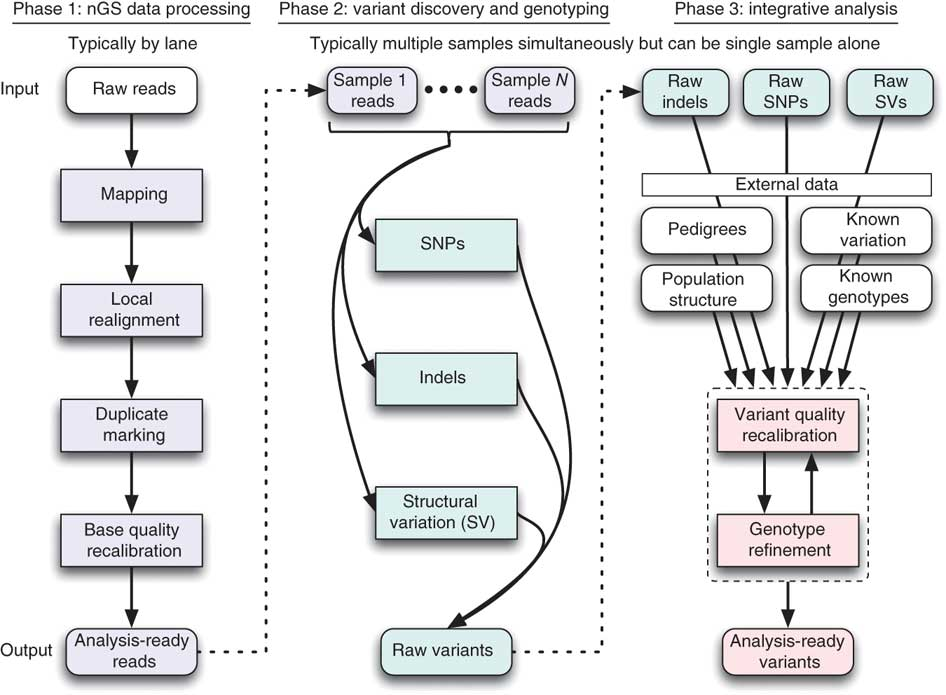
\includegraphics[width=\textwidth]{ng.806-F1.jpg}
\centering
\caption {NGS Workflow\autocite{depristo2011framework}.}
\label{fig:ng.806-F1.jpg}
\end{figure}


To be able to reliably carry out such analyses it is desirable for a system to have a number of capabilities that define the "workflow" of execution steps. These are:

\begin{itemize}
\item Define a structure that encodes a sequence of steps and the conditions for moving from one step to the next.
\item Ensure deterministic behaviour where possible i.e. same inputs produce the same output when run multiple times (whether in the same computational environment or different environments).
\item Ensure that the analysis has a finite run-time where possible.
\item Allow fine-grained control over the analysis configuration. 
\end{itemize}

\subsubsection{Workflow Structure Definition}
An effective and commonly utilized method of representing a workflow in the scientific analysis and other contexts is as a directed graph. Each vertex in the graph represents a particular computational step that needs to be carried out, and graph edges represent, possibly conditional, transitions between the vertices. This representational method allows the user to comprehensively express both the steps involved in an analysis, as well as specifying their sequence and executing control flow. Furthermore, the graph-based approach allows for a graphical representation of the workflow structure that is readily comprehensible by humans, thus increasing its utility. In general, the following requirements need to be met in order for the graph-based workflow representation to be fit-for-use in the scientific analysis context:

\begin{itemize}
\item The workflow should be encoded using a language and format that is easily readable by humans.
\item It should be possible to pass parameters to a workflow -- values that can be used at runtime to affect workflow behavior.
\item A workflow state should be able to invoke any program that is installed on the machine that is running that workflow state.
\item A workflow state should be able to interrogate the environment that it is running on i.e. check for presence/absence of certain files, communicate with a database, access URLs on the Internet.
\item Any number of transitions should be able to enter or leave a state.
\item It should be possible to render a graphical representation of the workflow as an image.
\item It should be possible for different states in a workflow to exchange information.
\end{itemize}

\subsubsection{Deterministic Behaviour}
Scientific reproducibility is a key concern that needs to be maintained in order for the system to be usable in the context of scientific analysis. Reproducibility, specifically, refers to the requirement for a user to be able to produce the exact same result as reported by another user using the same workflow definition, input files, and computing environment. While certain algorithms that may be executed as part of a workflow state like Expectation Maximization\autocite{moon1996expectation}, or Stochastic Gradient Descent\autocite{bottou2010large} behave in a non-deterministic manner where exact reproducibility of results may not be possible, the workflow system itself should not introduce any stochastic components when encoding workflow structure.

\subsubsection{Finite Run-Time}
The directed graph structure allows for transitions back to a previously visited vertex, thus creating graph cycles. Although this improves the expressiveness of the structure it is generally undesirable in the context of workflows as such a workflow may end up in a perpetual loop within the cycle requiring human intervention to diagnose and rectify at run-time. Although it is generally impossible to guarantee a finite run-time for a workflow due to the possibility of any underlying computational algorithm itself getting stuck in a perpetual loop or resource deadlock, we would like to rule out such a possibility at least from the perspective of workflow structure. Thus, we place an additional constraint on the workflow definition to be a Directed Acyclic Graph (DAG). Although this complicates somewhat the encoding of use cases where certain tasks need to repeated a number of times, these use cases are generally still attainable via programmatic generation of a series of states or using sub-graphs and gives us the added comfort of ruling out infinite loops where possible.

\subsubsection{Analysis Configuration}
A scientific analysis typically needs to be configured and parameterized at multiple levels. When considering different types of parameterization required, 3 distinct levels of parameterization can be identified. These are:

\begin{description}
\item[Workflow level] -- configuration that applies to a particular workflow regardless of which analysis it is used on. This may include things like paths to the location of certain programs used by the workflow, or their general invocation strings, or certain reference values.
\item[Analysis level] -- this includes values that may be different from one analysis to the next but are not different between samples under the same analysis.  Examples of such configurations are: common flags to pass to tool invocations, where to store analysis results, where to look up reference data sets.
\item[Execution level] -- these parameters differ even from one invocation of a given workflow under the same analysis to the next invocation. The most common instance of such a parameter is the set of names of input files that need to be processed by the workflow representing one sample. 
\end{description}

It is natural to view these configuration levels as a three level hierarchy where Analysis configurations expand on and override Workflow level configurations, and Execution level configurations expand on and override Analysis level configurations.

In order to successfully configure the workflow system it is necessary to be able to specify and permanently store such configurations in a format that is both human- and machine-readable. Thus, a user who is conceiving a particular analysis should be able to author a set of configurations that embody the nature and specifics of the analysis being performed. These configurations should then be easily transferrable to another individual or system instance for reproducibility purposes. Once the configuration of the system is fully specified the user should be able to launch their analysis according to this specification.

At run-time, the workflow system should be able reconstruct one \emph{effective} configuration from all levels of the configuration hierarchy and apply it appropriately.

\subsection {Workflow Engine} \label{sec:workflow_engine}

A Workflow Engine is necessary for the set of workflow definitions to be executable on a compute cluster. This workflow engine needs to be able to fulfill the following broad set of requirements:

\begin{itemize}
\item Workflow parsing and translation
\item Workflow state management
\item Workflow scheduling
\item Workflow execution
\end{itemize}

\subsubsection{Workflow Parsing and Translation}

While a workflow itself encodes the structure and sequence of computational steps that need to be performed, the workflow engine needs to be able to parse such a workflow definition and translate it into a set of commands that can be runnable on a real machine. To aid scalability it is desirable for the workflow to be broken down into a set of tasks at this stage that can be run on different physical machines. The workflow engine then needs to be responsible for producing this set of uncoupled commands from a monolithic workflow definition.

\subsubsection{Workflow State Management}

Workflow state management encompasses concerns of how to keep track of workflow definitions, including their versioning, as well as the status of various workflow instances. The workflow engine, then, needs to keep a registry of workflow definitions where, along with the workflow code and an identifier, the user can record useful metadata related to that workflow, such as - workflow version, author, owner, creation date, whether the workflow is enabled, etc. This registry is the authoritative source of information on what workflow capabilities a particular deployment of the workflow system has, and every new workflow, or update to an existing workflow must be recorded within this registry.

Furthermore, a particular version of a workflow definition may give rise to any number of workflow instances i.e. particular invocations of the workflow on a set of inputs and within the context of an analysis. Each instance may be in one of a number of different states, such as - Stopped, Running, Queued, Completed, or Failed. The workflow engine is responsible for keeping track of all of the workflow instances for a given workflow, and their states, and is responsible for transitioning the workflow instances from one state to the next, based on the preconditions for each such transition. These state transitions are not to be confused with the state transitions that are encoded within the workflow definition, as the workflow definition state transitions are custom to each workflow and encode the logic of the underlying scientific analysis, whereas the workflow instance state transitions and their conditions are standard for all workflows and workflow instances and describe the general workflow lifecycle. As with the metadata  recorded for workflow definitions, the workflow engine should also record metadata associated with workflow instance state transitions, the most important of which is the time-stamping of all such transitions. 
   
\subsubsection {Workflow Scheduling}

Once a workflow definition is parsed and translated into a series of runnable tasks, the workflow engine needs to be able to schedule these tasks for execution as appropriate. A Scheduler component within the engine needs to be able to match up two sources of information - availability of computational resources, and availability of runnable tasks, to produce a schedule i.e. a set of task-to-resource assignments within an appropriate timeframe. In order to accomplish this the Scheduler needs to be able to carry out a number of tasks, as detailed below.

To ascertain availability of computational resources the Scheduler needs to be able to communicate with all machines within the cloud computing cluster that are designated for running tasks. Furthermore, the scheduler needs to be able to interrogate the state of these machines to determine what the current level of load on each machine is, and whether the machine can accept more load in the form of new tasks. As the load level of each machine is of a dynamic nature, and is based on the completion of currently running tasks, the Scheduler needs to be in a constant state of communication with the entire compute cluster, in order to maintain an up-to-date picture of resource availability.

To establish a list of runnable tasks the Scheduler needs to iterate over all currently running workflows and determine the state of execution within them. As tasks are completed within each workflow instance, other tasks that are downstream from them in the workflow definition may become runnable. The scheduler should then determine for each workflow instance what its set of currently runnable tasks is, based on the structure of each workflow definition and the current state of the workflow instance.

One important concern within the realm of workflow scheduling is the concept of workflow and task priority. It is natural to think that not all workflows, and not all workflow tasks have the same priority i.e. some are more important than others and should, thus, have precedence when it comes to scheduling. It is then important for the Scheduler to be able to incorporate the concept of priority into the task scheduling decisions that it is making in order to meet user requirements.

Armed with a prioritized list of runnable tasks and a list of available resources the Scheduler needs to produce as set of task-to-resource assignments that can be used for workflow execution.

\subsubsection {Workflow Execution} 

The purpose of a workflow engine, at its core, is to execute workflows, thus, a set of execution capabilities is required. The sections above describe the requirements for parsing and translating a workflow into a set of runnable tasks, managing their state, and scheduling task execution according to its priority and resource requirements. The Execution component of a workflow engine needs to handle the actual running of tasks that have been scheduled.

Each machine in the cloud computing cluster that is part of the workflow system needs to be able to accept from the workflow scheduler a task execution assignment that encodes the details of the actual task that needs to be run. The task itself may consist of any number of computational steps. The Execution component is then responsible for transitioning a task from the Scheduled state to a Completed or Failed state, and carrying out the computational steps encoded within the task definition. This typically involves running other programs, collecting their return statuses, and execution timestamps and relaying this information to the Workflow State Management component.

When the Execution component encounters errors during task runtime it should be able to not only collect comprehensive information about the error condition, but should also be able to retry running the task without necessarily failing the overall workflow instance.
   
\subsection {System of Record} \label{sec:system_of_record}

One of the key requirements for a workflow system to be used in a scientific context is reproducibility. This concept was referenced earlier when describing the desire for a workflow to behave deterministically where possible. Another important factor that affects reproducibility is the method by which the course of a scientific analysis is encoded. We thus need an accurate system of record that keeps track of the following information:

\begin{itemize}
\item The various analyses that are undertaken
\item Workflows that are executed as part of each analysis
\item Samples that are part of the analysis
\item Overall system configuration
\end{itemize}

For each of the items above it is important to capture and permanently store a number of vital fields such as names, and unique identifiers, owner, version, and timestamp. Then, when the results of such an analysis are used in a scientific publication it is enough to provide the unique identifier of this analysis to be able to recover the technical details that will aid in reproducing analysis results by a 3rd party.

\subsection {Troubleshooting Errors} \label{sec:troubleshooting}

One of the inevitabilities of large scale computing is the occurrence of error conditions. The probability of an error being encountered in a unit of time increases together with the complexity of an analysis being performed and the amount of computational resources being utilized. In a traditional HPC-based scientific computing centre responsibilities for detecting and handling errors are divided between the end user who is responsible for errors that occur in their data or algorithms, as well as their encoding of cluster compute jobs, and the cluster IT personnel who are responsible for any errors that are caused by the overall software and hardware infrastructure failures. 

Although, it appears as if this division of responsibilities favours the end user by relieving them of the need to handle infrastructure issues, it has a notable downside. The underlying infrastructure and run-time environment are opaque to the end user who is only free to submit compute jobs and collect their results. On the other hand, the majority of errors (of any kind) manifest themselves as compute job failures and it is up to the end user to discern which of these are problems of their algorithm and which are problems of the infrastructure. Because of the opacity of the runtime environment, the end user has few tools at their disposal to be able to accomplish this task effectively and can spend significant effort troubleshooting issues that are outside of their domain of responsibility before being able to hand the incident resolution over to IT.

By contrast, in a cloud computing environment the end user has ownership of the health of the entire virtualized system including the infrastructure and the workloads that are running on it. This alleviates the issue of environment opacity described above but places a slew of new requirements on the operator of such a system when it comes to management of error conditions. Methods for detection and handling of errors differ depending on the source of the errors and we describe these in further detail below.

In general the following sources of error are identifiable and require appropriate handling:

\begin{itemize}
\item Errors within underlying scientific algorithms or the data they operate on
\item Errors within the workflow definition
\item Errors within the workflow engine
\item Errors within the virtual infrastructure
\item Errors within the bare metal hardware/software infrastructure and virtualization layers
\end{itemize}

\subsubsection {Errors Within Algorithms or Data}

Most scientific software is experimental by its nature and is developed by relatively few individuals compared to industry software, thus it is reasonable to expect that error conditions should occur within such software with a higher frequency than within mature and stable enterprise software. There are two standard mechanisms by which a program can return error conditions (whether they arise due to an error within the program or bad data) -- return value, and log files. Both of these should be collected to have the most accurate representation of the state of running algorithms.

Additionally, multiple algorithms running on the same virtual machine will compete for its limited resources and sometimes, despite best resource planning efforts, will deplete them, with adverse effects on system performance. For instance, a system that runs out of physical memory may start using virtual memory and causing excessive memory swapping, thus severely degrading performance. Although some of the information necessary to diagnose such conditions may be available via system logs, it is definitely not comprehensive, and will typically allow the operator to deal with issues in a reactive rather than proactive manner. It is desirable, instead, to be able to actively monitor the trends in resource utilization within the cloud computing cluster and deal with potential resource bottlenecks before they arise.

The most typical resolution strategy for errors of this type would be to fix the underlying algorithm and re-run it for all, or only the affected samples under study.

\subsubsection {Errors Within the Workflow Definition}

When creating workflows it is possible to introduce errors that will only manifest themselves at runtime. Such errors will typically either cause a workflow task to fail, thus failing the entire workflow, or will cause a workflow task to stall, preventing further progress. The workflow engine needs to collect information about all failures and present it to the end user on a management interface, as well as recording it in the engine log files. Information about typical task runtimes should also be recorded to aid identification of tasks that have stalled.

Such errors would typically be addressed by fixing the workflow definition and issuing a new version of the workflow that will need to be re-run on all samples.

\subsubsection {Errors Within Workflow Engine}

As the workflow engine consists of a large number of running programs, any number of these may encounter error conditions during their operation. Each program should have a log file where such information can be gathered.

These errors would typically be addressed by patching the workflow engine or possibly restarting services that got into a bad state and the workflows that are mid-flight need to be resilient to such a situation.

\subsubsection {Errors Within Virtualized Infrastructure}

A cloud computing cluster may consist of hundreds of Virtual Machines, each machine in turn running hundreds of programs simultaneously. Given the large size of the computational fleet it is not uncommon for entire Virtual Machines or significant components thereof to fail, either by issuing an error signal or simply by becoming unresponsive or unreachable on the network. A key source of information about error conditions at the machine level is the operating system log file and it should provide the necessary diagnostic information when an error signal is present. For the cases when this signal is not present, however, and a VM simply stops responding a more active monitoring system is required -- one that will periodically communicate with a Virtual Machine and collect its vital stats.

Errors within the VM Infrastructure are typically resolved by either patching and restarting services on the affected VM or by terminating and recreating the VM from scratch. The workflow system needs to be robust to both of these resolution strategies requiring only a minimal amount of work to be redone.

\subsubsection {Errors Within Bare Metal Hardware/Software}

As all cloud computing clusters represent virtualized hardware that is running on some bare metal server in a particular data center it is sometimes the case that the underlying hardware or software fails, thus rendering the Virtual Machine unusable. It usually not possible for a cloud end user to gain visibility into the bare metal layer, and the responsibility for detecting and handling such issues generally falls on the cloud operator. From the user perspective the VM simply fails or stalls, and although the user requires methods for detecting such conditions, the resolution strategy is typically to recreate the VM again. The size of the data center for a typical cloud provider is such that if the underlying issue only affects one or a small number of bare metal servers, the probability of the new VM being scheduled on an affected server for the second time is quite low and, thus, computation may resume normally. When large scale network or other hardware issues affect the entire data center it may be necessary for the user to tear down and recreate the entire cloud computing cluster.

Depending on the magnitude of the issue in question, the resolution strategy may involve recreating individual VMs or the teardown and re-creation of the entire workflow system. In order to avoid significant data loss in this case effective data backup and recovery strategies are required on behalf of the workflow system operator.


Based on examining the typical sources of errors at various layers of the system above, the following error detection and mitigation mechanisms can be identified:

\begin{itemize}
\item System Monitoring
\item Management Interfaces
\item Log Files
\end{itemize}

\subsubsection {System Monitoring}

As previously noted, error conditions often do not occur spontaneously but instead are a result of contention for finite resources by various programs, or a byproduct of events outside the scope of the workflow system itself. Moreover, error conditions do not always result in program crashes that can be recorded to a log, but can instead cause a system to stall, become unresponsive, or unreachable on the network. If the underlying cause of the issue is identified in time before the system reaches a critical state it is at times possible to gracefully recover from the situation without reaching a crash and with minimal loss of work or productivity. To make this detection possible an active monitoring system is required to be deployed on the cloud computing cluster. The job of such a monitoring system is to keep track of all Virtual Machines that are part of the cluster and collect monitoring metrics indicative of the health of each.

The following set of key metrics need to be supported:

\begin{multicols}{2}
\begin{itemize}
\item CPU load
\item Memory load
\item Free memory
\item Page faults
\item Swap size
\item Free disk
\item Disk latency
\item Disk throughput
\item Disk IOPS
\item Open files
\item Network latency
\item Network throughput
\item Number of open sockets
\item Number of database clients
\item DB Transactions per second
\item Transaction rollbacks
\item DB number of connections
\item DB Error count
\item HTTP errors
\item Queue size
\item Queue spillover
\end{itemize}
\end{multicols}

In order to be able to detect minute conditions that adversely affect the health of the cluster the monitoring system needs to sample all of the above metrics from each VM with a sub-second frequency. Furthermore, to enable detection of trends in system health, the monitoring system needs to retain collected data over a period of time that is as long, or longer, than a typical workflow execution time (which in the case of scientific workflows can be days or even weeks). Since a Virtual Machine that is experiencing an error condition may become sluggish or entirely unresponsive it is instrumental that the metrics data that is being collected for each machine is quickly shipped off to another machine that can house and aggregate all such data across the cluster. 

In order to allow end users to make use of the collected metrics for decision making the monitoring system needs to have graphing capabilities so that evolving trends in system health are made most evident. A set of graphical dashboards should be available to the user that demonstrate current and past cluster state based on the metrics above and a configurable time horizon. These dashboards will then be used during the course of system operation to identify potential issues and guide preventative or mitigative measures.

\subsubsection {Monitoring Alarms}

Because actively monitoring cluster state for potential issues via a set of dashboards is a time consuming task that may be prone to errors on behalf of the human observer an additional layer of the monitoring system should provide automatic notifications to the end user when the system enters a dangerous state such as high memory usage or CPU thrashing.

The user should be able to define a set of rules that express the conditions that are indicative of a system issue and require human intervention. Each rule should specify a metric or set of metrics, a set of thresholds, and an action. The monitoring system should continuously evaluate the metrics specified in each rule against the specified threshold, and when the metric value breaches the threshold the system should raise an alarm with the end user via the specified action. 

Because large scale events like network outages may cause many metrics to breach their stated thresholds at the same time the Alarm System should aggregate all similar events into a single event, where possible, to avoid overwhelming the end user with notifications that all have the same root cause.

\subsubsection {Management Interfaces}

Keeping track of the various moving pieces of a distributed workflow system requires a set of management interfaces so that the user can get an overview of overall system state and maintain control of the system. Such interfaces should show all of the Virtual Machines that are part of the cluster, what capabilities each machine has, what workflows are currently active, and state of any databases or queues that are part of the system. When error conditions occur within a particular sub-system, such as during the execution of a workflow task, these errors should be made visible on the corresponding management interface for that sub-system, along with any relevant details related to the error. Thus, a workflow management interface should show any failed tasks and provide remedial options to the user, directly on that interface, such as retrying or deleting a particular task or rescheduling the entire workflow. An interface that displays Virtual Machines should indicate when any of the VMs become unreachable or unresponsive and allow the user to delete and recreate the VM.

\subsubsection {Log Files}

As is evident from previous sections that describe possible sources of errors in the system, one of the most frequent mechanisms for recording error conditions is writing to a log file. While every Virtual Machine has a system-wide log file that contains error messages from many applications it is also customary for most applications to write their own log files. Since the workflow system consists of many components, many log files will get generated. Making use of the bulk of log data is typically produced by a large size cloud computing cluster is a major problem.

In order to make the log data usable to the system operator it is required to harvest and aggregate all relevant logs from each VM that is part of the compute cluster. Since a VM may become unresponsive due to an error condition and the information on this condition may reside in a log file, it is necessary to run an agent on all VMs that will periodically ship the logs to another location for aggregation. The storage location for logs should have substantial capacity, as a large scale cloud computing cluster can generate many TB of logs per day.

The logs need to be parsed according to their format and information relevant to any conditions of interest should be extracted, along with necessary metadata, such as the host IP address and timestamp. The parsed output should then be aggregated by error condition to produce summary, as well as detailed, reports to present to the user in the form of dashboards. Parsed log information should be indexed and retained for further querying when a user decides to investigate a particular issue they discovered via the dashboard.

\section{Non-functional Requirements} \label{sec:non_functional_requirements}

Alongside the functional requirements for the system that have been detailed in the previous section there are a number of non-functional requirements that need to be considered. Chief among these are:

\begin{itemize}
\item Scalability
\item Availability
\item Ease-of-use
\item Interoperability
\end{itemize}

\subsection {Scalability} \label{sec:scalability}

A major reason for utilizing cloud technologies for scientific computing is the need to compute over large data sets, ones that would otherwise be impractical or extremely costly to compute over. Thus building a system that can scale with the demand for computational resources is one of the key non-functional requirements for a successful scientific workflow framework. It is worth noting, that given cloud computing's prevalent cost model of charging for usage by the hour or minute it is equally important to be able to scale the system in both directions i.e. up when about to launch a massive compute job, and down when the major computation is finished, in order to operate the system in a cost-effective manner.

For purposes of scalability the workflow framework can be thought of as consisting of two types of components, which scale due to different factors:

\begin{description}
\item [Worker VMs] - These Virtual Machines are the computers that are responsible for running actual scientific algorithms that are encoded within workflow tasks. Different configurations of worker VMs may be required depending on what type of algorithm is invoked - ones with more RAM, CPU, disk, etc. The number of worker VMs required scales with the resource demands of each workflow and the number of samples that are under analysis. The majority of VMs on the cluster will be of this type. When no active workflows are present all worker VMs can be destroyed. Creating new worker VMs when the need arises should also be very easy within the workflow system.
    
\item [Control VMs] - Control VMs are Virtual Machines that are responsible for housing the various control components of the workflow system such as the Workflow Scheduler, Metrics Store, Management UIs, etc. Depending on the function served by each Control VM it can scale based on the number of Worker VMs, granularity of workflow tasks, or number of users of the system. Although it should be possible to scale the number of Control VMs up and down depending on need, a baseline number of Control VMs will be running for the duration of the cluster lifetime.
\end{description}

Based on the different types of components that compose the workflow framework the following scaling use case can be identified and need to be handled:

\begin{itemize}
\item Bootstrap a new installation into a minimal working configuration
\item Scale up worker fleet to meet anticipated resource demand increase
\item Scale down worker fleet to match resource demand decline
\item Scale up control VMs to meet anticipated resource demand increase
\item Scale down control VMs
\item Destroy entire compute cluster
\end{itemize}

\subsubsection {Bootstrap New Installation}

When installing on new clouds or Availability Zones it should be possible to easily install a basic working system with all of the necessary control and worker VMs to be able to handle some minimal amount of computational load. 

Of key importance is the distinction between systems that scale horizontally and systems that scale vertically. For systems that scale horizontally, it is relatively easy to scale up by adding new machines. Systems that scale vertically, such as database servers, do not easily allow adding new machines and instead require upgrading the resources within a single machine in order to scale up. It is generally more challenging and time consuming to scale vertically than horizontally.

When specifying a minimal installation it is important to set up those machines that scale vertically to a size that is larger than what is required by minimal system usage in order to avoid having to perform frequent upgrades. All databases and data stores fall into this category because of the complexity of upgrading the underlying storage once that database is in service.

\subsubsection {Scale Up Worker Fleet}

When the workflow framework is required to be able to perform more computation per unit time than it currently can, it should be easy to scale up the worker fleet by any number of VMs without interrupting existing jobs or requiring code changes. 

\subsubsection {Scale Down Worker Fleet}

When demand for computational resources wanes, it should be easy to destroy any number of idle worker VMs without interrupting presently running jobs or requiring code changes in order to minimize operating costs.

\subsubsection {Scale Up Control VMs}

Based on an increased number of worker VMs or increased number of users of the system it should be easy to scale up the Control VMs to maintain smooth operation of the cluster.

As before, it is important to delineate between vertically and horizontally scaling systems. For horizontally scaling systems, such as web-servers or distributed queues, scaling up may require bringing up a second or third server and setting up a load balancer. For vertically scaling systems, scaling up means migrating the existing system to a larger VM (with more memory, or cores), or migrating an existing data store to a larger storage device. Thus, as before, when scaling up vertically scalable systems, it is important to scale up appropriately to be able to handle all foreseeable, not just immediate, usage.

\subsubsection {Scale Down Control VMs}

Most Control VMs (for instance those serving data stores) tend to only grow in size, thus not ever requiring scaling down. It should be possible, however, to scale down certain components, such as web servers hosting management UIs, when a prolonged period of low activity is anticipated.

\subsubsection {Destroy Cluster}

When a long period of downtime is expected it may be required to destroy all of the active VMs in order to avoid paying for underused resources. A process should exist for detaching and conserving all of the active data stores, so that they can be reattached during the next bootstrap. All the appropriate configurations that are necessary for bootstrap should also be retained. At that point it should be safe to terminate all active VMs. 

\subsection {Availability} \label{sec:availability}

Availability refers to the definition of the circumstances under which the system as a whole, or its components, are able to perform their intended duties.

Although a scientific workflow system is an important computational aide it typically does not constitute a life-critical device that has extremely high availability requirements, such as those that might be found in a hospital life-support, or aeronautical system. Nevertheless, it is reasonable to expect that under normal operation, the system will be functional on a 24 hour, 7 days a week basis, and this intended schedule should inform system design.

Additionally, the following concerns regarding Availability should be considered:

\begin{itemize}
\item Service Redundancy
\item Service Upgrades
\item Backup and Disaster Recovery
\end{itemize}

\subsubsection {Service Redundancy}

Some components of the workflow system are such that if they crash or go offline, the system will continue functioning, although, perhaps, in a reduced capacity - Metrics Monitoring, and Log Aggregation are examples of such components. Other components, like Workflow Scheduler, Workflow State Management, and others, were they to go down, would bring down the entire operation. Thus, in order to maintain service availability during adverse events, it is important to build service redundancy into the design of the system.

Typically, Service Redundancy takes the shape of having a second standby server that is able to stand in place of the main server if it was to go offline. Multiple levels of standby are available, and should be used as appropriate:

\begin{description}
\item [Cold Standby] - Set up the backup machine when primary machine fails.
\item [Warm Standby] - Backup machine is set up and will be powered on when primary machine fails.
\item [Hot Standby] - Backup machine is set up and powered on, traffic will be diverted to it when primary machine fails.
\item [Both Active] - Both primary and backup are actively serving traffic in a load balanced manner. 
\end{description}

\subsubsection {Service Upgrades}

Upgrading software is the leading cause of planned service outages. From a customer perspective, although the disruption is planned, and warning can be given, it is still a disruption and thus should be avoided where possible. 

It is not always possible to upgrade software without a service interruption, but utilizing standby servers and appropriate load balancers can increase the number of deployments that are performed without a disruption to the users. Thus, service upgrades should be scripted such that a backup server is brought online, to which active traffic will be diverted by the load balancer while the main service is upgraded. Once the main server is upgraded, the load balancer should switch traffic back and allow the backup server to be upgraded, and brought back offline where appropriate.

\subsubsection {Backup and Disaster Recovery}

In the event of a catastrophic system failure it should be possible to recover as much of the data as is warranted by the scientific use case the system is being utilized for, and resume normal operation as soon as possible. Data backup and recovery procedures should be put in place for all of the main data stores, especially those housing workflow scheduling and state management facilities as loss of these may potentially mean not only redoing the in-flight analyses but also past ones, as otherwise reproducibility would be lost.

\subsection {Ease-of-use} \label{sec:ease_of_use}

Cloud computing is a relatively new technology and coupled with the complexity of a distributed workflow system can create a learning curve that would hinder system adoption. To help potential users through the learning curve and encourage a wider adoption of the product the following measures are required:

\begin{itemize}
\item Detailed User Guide
\item Detailed code comments
\item Standardized code style
\item Hands-off operation where possible
\item Contextual help
\item Intuitive Management UI
\end{itemize}

\subsection {Interoperability} \label{sec:interoperability}

Because data needs to be fed into it and results need to be retrieved out of it, a cloud based distributed workflow system does not exist in isolation from the rest of the world. Thus, a level of interoperability is required whereby systems upstream and downstream from the workflow framework need to be able to successfully interact and exchange information with the framework.

The most common need for interaction is when feeding data into the system. Since sample management is a complex issue on its own it falls outside of the scope of requirements for the workflow framework and typically resides within the realm of Laboratory Information Management Systems or Data Repositories. Yet, samples needs to be made available to the framework in order to enable computation. Thus, the framework needs an interface whereby locations of samples under analysis can be specified.

Another use case for interoperability is the desire to make the framework amenable to automation via scripting, so that, for instance, new samples that come into the laboratory can be automatically scheduler for a battery of standardized workflows to be performed, or a new algorithm version becoming available will automatically trigger a re-running of all samples under study using the new tool.

In order to enable this level of interoperability a set of APIs must be developed that provide all of the main framework operations through an interface that another program can interact with.

User Interfaces developed for the framework should utilize the same set of APIs where possible for consistency purposes, and to ensure that API code is frequently executed.

\section{General Design Principles}
To address the need for a large-scale cloud-based distributed workflow system that is suitable to scientific computing applications we present the design of our framework called Butler - a software toolkit built to implement the requirements specified in the Requirements chapter of this document.

Although a detailed description of system Architecture and Design follows, we begin by describing several guiding principles that have been adopted in the design of this system:

\begin{itemize}
\item Existing Open-Source Software
\item Service Orientation
\item Cloud Agnostic
\item Open-Source License
\end{itemize}

\subsection {Existing Open-Source Software}

The scope of the requirements for a workflow system of the nature described in this work are quite vast and building such a system from scratch would take years of effort from an entire software team. On the other hand, many of the requirements of the system can be readily met via existing software products. Although commercial software products tend to have better technical support, in the interest of cost savings, and in order to keep the entire solution open source we have opted to use all Open Source Software components when building Butler.

Since keeping the amount of new code that needed to be written to build Butler to a minimum was one of the cornerstones of system design, a very substantial portion of the overall system consists of 3rd party OSS frameworks that are integrated together to produce Butler. These include:

\begin{itemize}
\item Hashicorp Terraform\autocite{Terraform_by_HashiCorp_2016-10-31} (https://github.com/hashicorp/terraform) - for Cluster Lifecycle Management
\item Hashicorp Consul\autocite{Consul_by_HashiCorp} (https://github.com/hashicorp/consul) - for Service Discovery and Service Health Checking
\item Saltstack\autocite{SaltStack_2016-10-31} (https://github.com/saltstack/salt) - for Cluster Configuration Management
\item Apache Airflow\autocite{Apache_Airflow__2016-10-31} (https://github.com/apache/incubator-airflow) - for Workflow Management
\item RabbitMQ\autocite{RabbitMQ_2016-10-31} (https://github.com/rabbitmq/rabbitmq-server- for Queuing
\item Celery\autocite{Celery_2016-10-31} (https://github.com/celery/celery) - for Task Scheduling
\item Collectd\autocite{collectd_2016-10-31} (https://github.com/collectd/collectd) - for Metrics Collection
\item InfluxData InfluxDB\autocite{InfluxDB} (https://github.com/influxdata/influxdb) - for Metrics Storage
\item Grafana\autocite{Grafana.net} (https://github.com/grafana/grafana/) - for Metrics Dashboards
\item Logstash\autocite{Logstash} (https://github.com/elastic/logstash) - for Log Harvesting
\item Elasticsearch\autocite{Elasticsearch} (https://github.com/elastic/elasticsearch) - for Log Indexing and Aggregation
\item Kibana\autocite{Kibana} (https://github.com/elastic/kibana) - for Log Even Dashboards
\end{itemize}

These products were selected based on their ability to fulfill the specified requirements as well as their overall viability as Open Source projects. Viability was generally evaluated based on the following set of criteria:

\begin{itemize}
\item Number of Github stars
\item Number of repository contributors
\item Number of commits in the past year
\end{itemize}

At the time of writing (September 2016), these metrics are evaluated as follows:

\begin{table}[]
\label{tab:open_source_framework_viability}
\renewcommand{\arraystretch}{1.2} 
\centering
\caption{Open Source Framework Viability}
\begin{tabular}{@{}llll@{}}
\toprule
Product & Number of Stars & Number of Contributors & Commits in last 12 months\\
\midrule
Terraform & 5611 & 638 & 4543 \\
Consul & 7220 & 250 & 1129\\
Saltstack & 6850 & 1580 & 9769 \\
Airflow & 3419 & 178 & 1394\\
RabbitMQ  & 1964 & 63 & 1038\\
Celery & 5224 & 462 & 854\\
Collectd  & 1246 & 262 & 1104\\
InfluxDB & 8773 & 237 & 2299\\
Grafana  & 11666 & 320 & 2952\\
Logstash & 6405 & 348 & 598\\
Elasticsearch & 18285 & 691 & 6279\\
Kibana  & 5957 & 146 & 3409\\
\bottomrule
\end{tabular}
\end{table}

\subsection {Service Orientation}

One of the key requirements for Butler is Scalability i.e. the desire to be able to scale the amount of resources utilized by the framework up and down arbitrarily according to analysis needs. Applications that are monolithic in nature suffer from scalability issues due the large number of competing constraints within application components. To help alleviate this concern we take a Service Oriented approach in the design of the system. Butler is composed of a number of loosely coupled services each of which implements a particular function. Because the services are decoupled, each service can be optimized and scaled individually, according to user requirements. On the other hand, the complexity of the overall application is increased somewhat because of the need to deploy and manage separate services that are in communication with each other.

Another benefit of Service Orientation is the ability to independently upgrade components of the software without affecting other running components. As an example, the Collectd metrics collection component can be patched independently of the rest of the system, thus increasing system Availability.

\subsection {Cloud Agnostic}

Because of its early entrance on the cloud computing scene, the AWS Cloud by Amazon.com Inc currently enjoys a significant lead in this market segment, having over 31\% of the entire public cloud-computing market:

\begin{figure}[h]
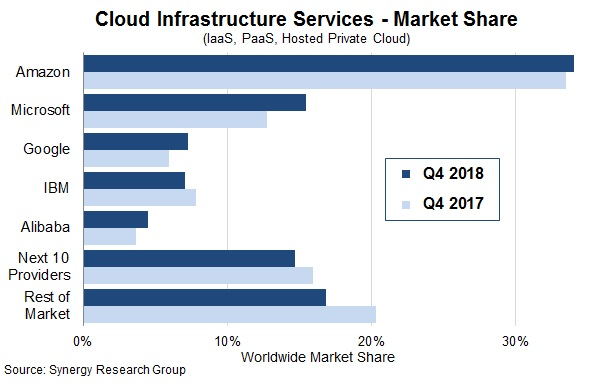
\includegraphics[width=\textwidth]{cloud_market_share}
\centering
\caption {Cloud market share by vendor}
\label{fig:cloud_market_share}
\end{figure}

Each of the top 4 cloud service providers - Amazon, Google, IBM , Microsoft, as well as smaller cloud providers that use the Openstack platform, provides not only the basic IaaS offering, but also an entire ecosystem of cloud based components - a PaaS, including networking, queues, databases, etc. Thus, it may be tempting to select one of these providers and build an entire software system that is based on a single vendor's offerings. This has the potential benefit of significantly simplifying system architecture and providing a single point of contact for troubleshooting.

It is, however, our opinion that taking such an approach would limit the appeal of the system to a wider user base. This opinion is driven by several considerations:

\begin{itemize}
\item The cloud computing market segment enjoys a great deal of growth and significant shifts in growth year-over-year as evidenced by Figure\ref{fig:cloud_market_share}, thus committing to a particular platform that is seen as a current market leader today, may limit the usability of the software when the chosen vendor falls out of the race in the future.
\item Because the market segment is highly competitive, end users can benefit significantly from limited time deals offered to them by cloud providers if they are flexible about what platform to deploy on.
\item Selecting one vendor induces vendor lock-in, possibly forcing adoption of inferior technologies to stay consistent with vendor choice.
\item Public and Private clouds typically operate on different software stacks. The nature of the data that is subject to scientific analysis may dictate where the analysis is able to proceed. 
\end{itemize}

On the other hand, supporting multiple cloud vendors has its own set of drawbacks:

\begin{itemize}
\item Handling multiple APIs for different vendors increases system complexity.
\item A solution that is vendor agnostic may lack certain capabilities that are only available to a subset of the vendors.
\item Some code duplication is inevitable when dealing with multiple platforms.
\end{itemize}

Based on considerations above we have taken the path of creating a cloud-agnostic system, i.e. one that will run on any major cloud providers, public, or private.

\subsection {Open Source License}

We adopt an open-source GPL v3.0 license for Butler.

\subsection {Overall System Design}

Overall, the Butler system can be thought of as being composed of four distinct sub-systems, each of which fulfills a number of requirements from Section \ref{sec:functional_requirements}. These sub-systems are:

\begin{description}
\item [Cluster Lifecycle Management] - This sub-system deals with the task of creating and tearing down clusters on various clouds, including defining Virtual Machines, storage devices, network topology, and network security rules. It implements requirements from sections \ref{sec:access_to_data}, and \ref{sec:access_to_compute_capacity}.
\item [Cluster Configuration Management] - This sub-system deals with configuration and software installation of all VMs in the cluster. It implements requirements from section \ref{sec:algorithm_implementation}.
\item [Workflow System] - The Workflow sub-system is responsible for allowing users to define and run scientific workflows on the cloud. This sub-system implements requirements from sections \ref{sec:workflow_definitions}, \ref{sec:workflow_engine}, and \ref{sec:system_of_record}.
\item [Operational Management] - This sub-system provides tools for ensuring continuous successful operation of the cluster, as well as for troubleshooting error conditions. It implements requirements stated in section \ref{sec:troubleshooting}
\end{description}

Each sub-system is described in full detail below.

\section{Cluster Lifecycle Management}

Before any computation can happen on the cloud a cluster of Virtual Machines is needed. The scope of Cluster Lifecycle Management includes:

\begin{itemize}
\item Defining hardware configuration for VMs
\item Defining initial basic software configuration for VMs
\item Defining storage devices
\item Defining network topology
\item Defining network security
\item Creating and Tearing down VMs
\end{itemize}

Detailed requirements for these capabilities are specified in sections \ref{sec:access_to_data}, and \ref{sec:access_to_compute_capacity}.

To fulfill these requirements in a cloud agnostic manner Butler utilizes a framework called Terraform, developed by Hashicorp.

\subsection{Terraform}

Terraform is an Open Source framework for cloud agnostic cluster lifecycle management, that has been built by Hashicorp Inc., a San Francisco, California based company, and is distributed via a Mozilla Public License. The source code for Terraform is hosted on Github at https://github.com/hashicorp/terraform, and at the time of this writing (September, 2016) the latest release of the software is version v0.7.3

Terraform uses a proprietary human and machine readable file format for specifying cluster configurations that is called HashiCorp Configuration Language (HCL). Using this language the end user can define a number of constructs for cluster management, most important among them are - providers, resources, and variables.

\subsubsection {Terraform Providers}

Terraform providers enable the framework to talk to different cloud provider APIs. Each provider is responsible for translating HCL configurations into cloud-specific API calls. At the time of this writing the following Providers are available:

\begin{multicols}{2}
\begin{itemize}
\item AWS
\item CenturyLinkCloud
\item CloudFlare
\item CloudStack
\item Cobbler
\item Datadog
\item DigitalOcean
\item DNSimple
\item Google Cloud
\item Heroku
\item Microsoft Azure
\item OpenStack
\item SoftLayer
\item Scaleway
\item Triton
\item VMware vCloud Director
\item VMware vSphere
\end{itemize}
\end{multicols}

Typically in order to use a particular provider the user needs to insert a provider block into their configuration file where they specify details relevant to communicating with the particular API in question, such as - endpoint URL, username, password, SSH keyname, API key, etc., as seen in Figure \ref{fig:terraform_aws_provider}. 

\begin{figure}[h]
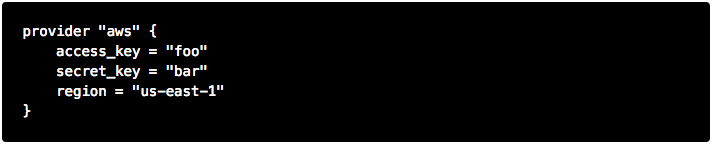
\includegraphics[width=\textwidth]{terraform_aws_provider}
\centering
\caption {Example Terraform provider configuration}
\label{fig:terraform_aws_provider}
\end{figure}

Once the user has specified a provider they can declare provider-specific Resources that define their cluster.

\subsubsection {Terraform Resources}

Resources represent different objects such as VMs, network routers, security groups, disks, etc., that the user can create on a given cloud. Each resource has a set of configuration options that can be specified to customize its behaviour. An optional \emph{count} attribute defines how many instances of the resource need to be created in the cluster.

\begin{figure}[h]
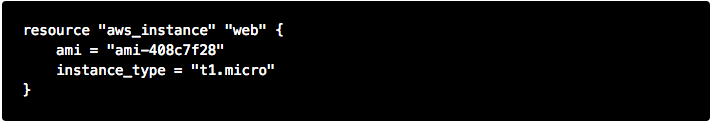
\includegraphics[width=\textwidth]{terraform_aws_instance}
\centering
\caption {Example Terraform AWS instance configuration}
\label{fig:terraform_aws_instance}
\end{figure}

Most Terraform configuration involves configuring resources.

\subsubsection {Terraform Variables}

Terraform variables are similar to variables in any other programming context. They consist of values assigned to labels, that can then be used for lookup elsewhere. Variables can be of string, list, or map type.

\begin{figure}[h]
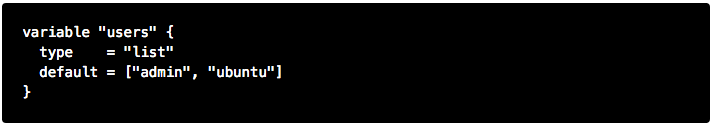
\includegraphics[width=\textwidth]{terraform_variable}
\centering
\caption {Example Terraform variable definition}
\label{fig:terraform_variable}
\end{figure}

Users typically specify variables in a separate configuration file and then use them throughout their cluster definition. 

One special case of using variables comes from specifying secret values such as passwords or secret keys that the use would not want to commit to a source repository. In this case, a variable can be referred to inside the configuration file, while being defined as an environment variable on the machine that Terraform will be executed on. The user prefixes the variable name with a special prefix -- \mintinline{sh}{TF\_VAR\_} which signals Terraform to parse the environment variable as a Terraform variable and allow appropriate substitution at runtime.

\subsubsection {Terraform Provisioners}

When a Virtual Machine is created the user may want to place certain files on it or run certain commands such as starting services or registering with a cluster manager, in order to bootstrap it. This purpose is served by Terraform Provisioners, which define code blocks that are executed on the target resource upon creation.

\begin{figure}[h]
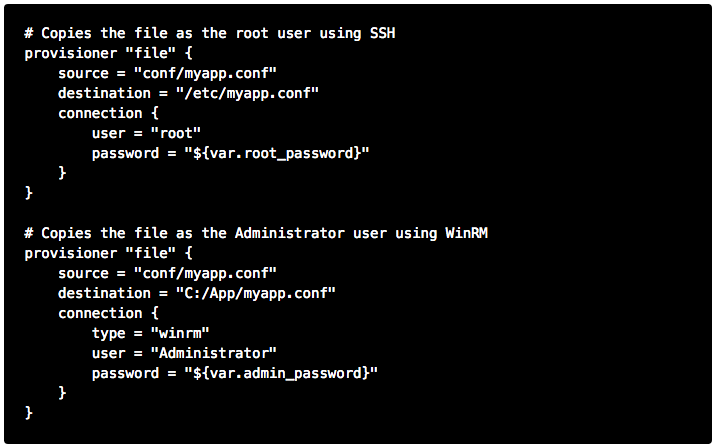
\includegraphics[width=\textwidth]{terraform_provisioner}
\centering
\caption {Example Terraform provisioner definition}
\label{fig:terraform_provisioner}
\end{figure}

\subsubsection {Terraform Installation}

Terraform is installed via a binary file downloaded from the Hashicorp website or by compiling the source code from github. It is a lightweight application that can be run from either the user's local machine, or from a special host on the target cloud environment. The application consists of a terraform CLI that the user can interact with by issuing shell commands. Typically users will combine their Terraform configuration files (stored in a source code repository) with a set of locally defined environment variables to set up and manage their clusters via the CLI.

\subsubsection {Terraform Cluster Lifecycle}

The key task of Terraform is to perform Create, Read, Update, and Delete on cluster resources. Create and Update operations are accomplished by issuing a \mintinline{sh}{terraform apply} command at the shell, while the shell is pointing to a directory with Terraform resource definitions. If the resources specified in the configuration do not yet exist, they are created. If the resource definitions have been changed since the last time \mintinline{sh}{terraform apply} was run, they will be brought into a state consistent with the latest definitions. This may involve updating existing resources where possible, or recreating them, where an update is not possible.

Terraform determines what changes need to be made in order to perform a successful Update via a file that is called a State file. This file specifies in a JSON format the current state of all infrastructure managed by Terraform. Running \mintinline{sh}{terraform apply} causes the tool to inspect current state and compare it to the target state, issuing any necessary commands to update current state to the target.

The Read operation simply displays the current Terraform state file via the \mintinline{sh}{terraform show} command.

The Delete operation is accomplished via the \mintinline{sh}{terraform destroy} command.

Other commands allow the user to validate the syntax of their configuration files, perform a dry run of resource creation, manually mark resources for recreation, and others.

\subsection {Terraform Use in Butler}

Butler comes with a set of Terraform configuration files that define templates for all of the VMs that constitute a functional Butler cluster, as well as configurations for network security. As previously stated a Butler cluster consists of Control VMs and Worker VMs - templates for both are available. The users are expected to adapt the templates as needed for their use case, providing their own credentials, cluster size, and other configurations.

\subsubsection {Example Configurations}


Listing \ref{lst:terraform_worker} demonstrates the Butler configuration file used to create 175 identical worker VMs that differ only by their hostname. 

The provider definition shows the procedure for setting up an OpenStack provider as well as demonstrating usage of variables where \mintinline{text}{user_name, tenant_name, and auth_url} are expected to come from a separate variable definition file, and  \mintinline{text}{password} is expected to come from an environment variable. 

The resource section shows definition of an OpenStack specific VM type \mintinline{text}{openstack_compute_instance_v2}, which has attributes like 
\mintinline{text}{image_id, flavor_name, security_groups, network}, etc. The  \mintinline{text}{connection} definition within the resource specifies how users will be able to connect to the newly created VMs. In this case it is accomplished via SSH using passwordless key-based authentication via a pass-through bastion host on the cloud.

Of further interest is the mechanism by which the creation of multiple instances of the same type is accomplished. The resource definition admits a \mintinline{text}{count} attribute which specifies how many instances need to be created. Furthermore, a \mintinline{text}{count.index} property keeps track of which instance is being created at run-time and can be used to provide unique hostnames to each instance as follows -   \mintinline{text}{name = "${concat("worker-", count.index)}"}.

Lastly, the \mintinline{text}{provisioner} section runs a set of commands that provide initial configuration for the new host upon first bootup. These include installing and running the Saltstack service which is used for configuration management, setting up machine roles  that determine what capabilities this VM will have in the cluster, and telling the VM what the IP address of the cluster manager is.

Listing \ref{lst:terraform_security_group} demonstrates the definition of a security group under OpenStack. VMs that are put into this security group will have two network security rules applied to them - opening port 22 for SSH communication between hosts, and opening ports 4505-4506 to enable Saltstack communication.

\section{Cluster Configuration Management}

Although a Cluster Lifecycle Management system like Terraform can create a Virtual Machine using a machine image, and even run some initial configuration commands, it is not enough to successfully manage the configuration of an entire large-scale computational cluster. Machines in the cluster will have hundreds of programs installed and configured on them, oftentimes with intricate interdependencies, and inter-machine communication requirements. Moreover, different operating systems will typically have different commands and mechanisms for installing and configuring software, and it would be unnecessarily limiting to require the end user to commit to a particular flavour of operating system. To help accomplish these tasks, as well as detailed requirements from Section \ref{sec:algorithm_implementation} we need to enlist the help of a Cluster Configuration Management system.

Several open source Configuration Management systems are available on the market today, the main options are:

\begin{itemize}
\item Chef
\item Puppet
\item Ansible
\item Saltstack
\end{itemize}

Each system has benefits and drawbacks and a dedicated user base. Table \ref{tab:configuration_management} compares the github codebases for these products in terms of number of stars, number of contributors, and number of commits in the last year. 

\begin{table}[H]
\renewcommand{\arraystretch}{1.2} 
\centering
\caption{Configuration Management Frameworks github summary}
\label{tab:configuration_management}
\begin{tabu} to \linewidth{XX[,r]X[,r]X[,r]}
\toprule
Product & Number of Stars & Number of Contributors & Commits in last 12 months\\
\midrule
Chef & 4417 & 474 & 1861 \\
Puppet & 4151 & 431 & 1474\\
Ansible & 18720 & 1469 & 3483\\
Saltstack & 6850 & 1580 & 9769 \\
\bottomrule
\end{tabu}
\end{table}

As can be seen from the data, all four are fairly active and stable projects, Ansible appears to be the most popular tool, and Saltstack is most actively developed, based on number of commits and contributors. Both Puppet and, Chef come from the first generation of configuration management tools having been initially released in 2005 and 2009 respectively, and suffering somewhat from having been trailblazers in the field. The largest complaint against both systems has been their unnecessary complexity and steep learning curve. Ansible and Saltstack, on the other hand, can be thought of as the second generation of configuration management systems, first released in 2012 and 2011, respectively. Both are based on simple to read and understand YAML-based configuration files, and have generally enjoyed greater adoption in the field.

For Butler we selected Saltstack to fulfill configuration management duties. The chief reason for selecting Saltstack over Ansible was that Saltstack appears to perform better when managing large clusters, whereas Ansible is known to suffer from increased lag in these scenarios. Since we anticipate to operate Butler clusters with several hundred VMs at a time we settled our choice on Saltstack.

\subsection {Saltstack}

Saltstack is an open source product that has been developed specifically for large scale configuration management. The key paradigm that Saltstack implements is declarative configuration management. This means that the user specifies declaratively, in a configuration file, what state a particular Virtual Machine should be in (in terms of installed and running software), and the Saltstack engine automatically compares the desired state to the actual state and carriers out the necessary actions to match the two. As an added benefit, it does so in an operating system agnostic manner. In contrast to scripts that operate in an imperative manner via statements like \mintinline{sh}{yum install apache} or \mintinline{sh}{service httpd start}, Saltstack files describe a desired state with statements like \mintinline{yaml}{service.running} and \mintinline{sh}{package.installed}. In the first case, the script would try to install the package a second time, even if it was present, whereas Saltstack first figures out whether the package is installed and only installs it if it is missing.

\subsubsection {Saltstack Architecture}

The Saltstack architecture consists of a cluster of Minions that are managed by one or many Masters. A Master is a Virtual Machine that acts as the authority on configuration definitions within the cluster and issues commands that the Minions run. A Master needs to have configuration definitions stored locally on its disk or be available through a git repository. It runs a special salt-master daemon, and requires certain network ports to be open for communication.

Minions need to know how to find the master on the network (by IP address). Each Minion generates a unique key and presents it to the Master. Once a Master accepts the Minion's key there is a handshake and the Minion falls under the Master's control. The Minion runs a salt-minion daemon.

Each Minion can have a number of roles assigned to it and the Master maintains mappings between roles and configurations. Once the Master has determined what roles a Minion has it can issue the necessary commands to apply relevant configurations to the Minion. 

\subsubsection {Saltstack Data Model}

The Saltstack Data Model has four main concepts - State, Pillar, Grain, and Mine. We consider each in turn.

\paragraph{A Salt State} is simply the definition for what state some piece of infrastructure should be in. For instance, if we want some server in our cluster to be in the state of running a PostgreSQL database we need to do the following:

\begin{enumerate}
\item Create a postgres user
\item Create a postgres directory
\item Download the postgres-server package
\item Install the postgres-server package
\item Initialize the database
\item Override default configuration settings
\item Start the server
\end{enumerate}

The corresponding Salt state that accomplishes the same task looks as follows:

\captionof{listing} {Salt state for setting up a PostgreSQL server. \label{lst:salt_state_postgres}}
\begin{minted}
[
breaklines=true,
linenos,
fontsize=\footnotesize,
frame=lines,
framesep=2mm,
baselinestretch=1.2
]
{yaml}
install_server:
  pkg.installed:
    - name: postgresql95-server.x86_64
    
initialize_db:
  cmd.run:
    - name: /usr/pgsql-9.5/bin/postgresql95-setup initdb
    - unless: stat /var/lib/psql/9.5/data/postgresql.conf

/var/lib/pgsql/9.5/data/postgresql.conf:
  file.managed:
    - source: salt://postgres/config/postgresql.conf
    - user: postgres
    - group: postgres
    - mode: 600
    - makedirs: True

    
start_server:    
  service.running:
    - name: postgresql-9.5
    - watch:
      - file: /var/lib/pgsql/9.5/data/*
\end{minted}

The code for a Salt state is placed in a special file called an \emph{.sls} file. All of the state definitions that the system knows about are arranged into a folder hierarchy where the name of each folder defines the name of the state. The state definition is then located inside the folder in a file named \emph{init.sls}, as demonstrated in Figure \ref{fig:salt_state_airflow} for the Airflow Workflow engine.

\begin{figure}[H]
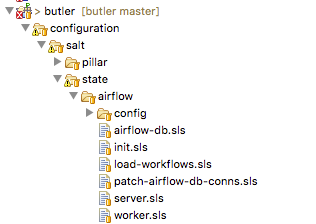
\includegraphics{salt_state_airflow}
\centering
\caption {Salt state files for Airflow Workflow Engine}
\label{fig:salt_state_airflow}
\end{figure}

Several related states (such as those describing different installations of the same program) can be grouped together under the same parent state. Then each sub-state is placed into its own \emph{.sls} file under the main state's folder, with the name of the file giving rise to that state's name. Figure \ref{fig:salt_state_airflow} provides an example of this scenario where in addition to the main \emph{airflow} state there are sub-states such as \emph{airflow.server}, \emph{airflow.worker}, \emph{airflow.load-workflows} etc. Note that sub-states are referenced via \emph{name\_of\_parent\_state.name\_of\_substate}.

\paragraph{A Salt Pillar} is a set of key-value pairs that are stored encrypted on a Minion and constitute look-up values that are relevant for that Minion's configuration. Examples of Pillar values can be usernames and passwords, locations of certain files, etc. A State definition can refer to Pillar values when configuring a system, and two identical VMs that differ only by their Pillar values will be parametrized differently at configuration time. One example of this is setting up the same server in a QA environment vs. Production. In QA the server may point to a test data directory with especially constructed data files, for testing purposes, whereas in Production the server would point to the actual data directory with real samples.

The Pillar are organized similar to States in a folder hierarchy of \emph{.sls} files. Figure \ref{fig:salt_pillar_hierarchy}

\begin{figure}[H]
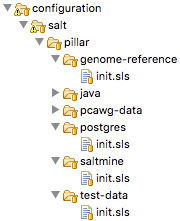
\includegraphics{salt_pillar_hierarchy}
\centering
\caption {A set of Salt Pillar definitions}
\label{fig:salt_pillar_hierarchy}
\end{figure}

Listing \ref{lst:salt_pillar_test_data} shows an example Pillar definition where information related to finding test data is stored.

\paragraph{Salt Grains} are bits of information Salt collects about Minion state or characteristics. They include things like:

\begin{itemize}
\item Minion IP address
\item Amount of RAM on minions
\item Minion hostname
\item Minion network interfaces
\end{itemize}

and others. The Grains can be used to introspect and pass on configuration values (like IP address) that are not known in advance. One of the most important uses of Grains is the ability to assign roles to a Minion via the Grains mechanism. Since roles define what states are eventually applied, adding or removing a role to a VM via Grains has a very significant side-effect. 

\paragraph{The Salt Mine} is a centralized repository of information about the state of all Minions that is stored on the Master. Information is passed into the Mine from Grains and other sources. It can then be used inside state definitions to further customize the system.  

Listing \ref{lst:salt_mine} demonstrates how the Jinja templating engine is used to look up the IP Address of servers in the cluster that have the \mintinline{text}{consul-server} or\mintinline{text}{consul-bootstrap} role. Then this IP Address is used inside a State definition to join a cluster of similar machines. Without the Mine, this particular Minion would not know who to ask for this IP Address, but because the Mine is centralized on the Salt Master host this lookup is possible.

\paragraph{The Top File} is the mechanism used in Saltstack to specify what VMs will have what States applied to them. The Top File provides a lot of flexibility in terms of how to accomplish this mapping. Mappings can be accomplished via hostname or any Grains values, and it allows regular expressions. The most flexible and, thus preferred, method of mapping States to VMs is via Roles.

Listing \ref{lst:salt_top_file} demonstrates how the State mapping to Roles is accomplished in a Top File. Based on this Top File all VMs will get the \mintinline{text}{consul, dnsmasq, and collectd} states. VMs with the \mintinline{text}{monitoring-server} role will get \mintinline{text}{influxdb, and grafana}, and VMs with the \mintinline{text}{job-queue} role will get the \mintinline{text}{rabbitmq} State.

\subsubsection{Controlling Saltstack}

Control over the cluster is exercised from the Salt Master. The user establishes a shell session on the Salt Master and issues commands via the Saltstack CLI. Each command has the following syntax:

\mintinline{text}{"salt target_expression command_expression"} where:

\mintinline{text}{salt} is the name of the Salt CLI.

\mintinline{text}{target_expression} is an expression that determines what VMs to apply the command to. It can be a logical expression that combines hostnames, grains, and regular expressions.

\mintinline{text}{command_expression} is an expression that determines what actual command to run on the targeted VMs. The \mintinline{text}{command_expression} can be as simple as running a shell command on the target VMs, or it can apply a particular named state via the \mintinline{text}{state.apply} command, or it can apply all matching states via the special \mintinline{text}{state.highstate} command.

For example, \mintinline{sh}{salt -G 'roles:worker' state.apply airflow.patch-airflow-db-conns} applies the \mintinline{text}{airflow.patch-airflow-db-conns} state to all VMs that have the \mintinline{text}{worker} role.

\subsection{Saltstack Use in Butler}

Butler uses Saltstack extensively in order to install software on the cluster. This includes software that is required to run Butler itself, as well as installing scientific algorithms required for running actual workflows on Worker VMs (as specified in Section \ref{sec:algorithm_implementation} of the Requirements chapter). As seen in Figure \ref{fig:salt_states} the Saltstack configuration in Butler consists of a set of State and Pillar definitions along with the Top Files that map these States and Pillar to various VMs in the cluster. These definitions are enough to configure a completely functional Butler cluster from a single shell command.

\begin{figure}[H]
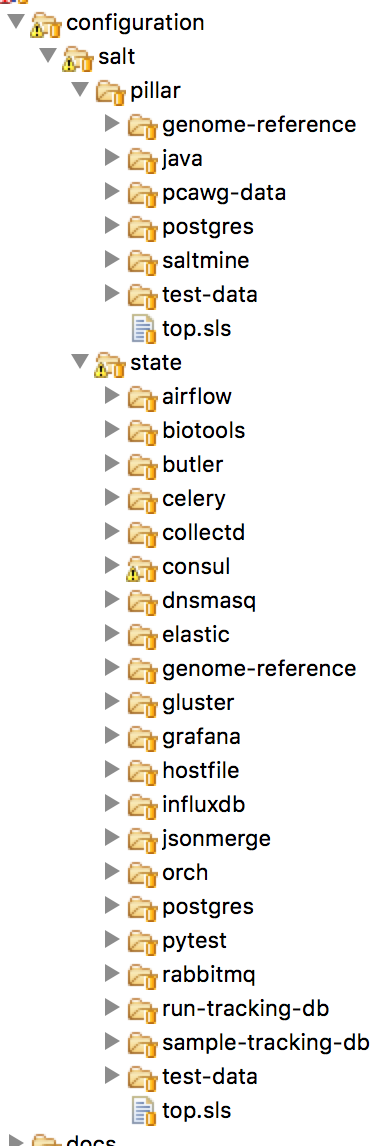
\includegraphics{salt_states}
\centering
\caption {Salt States and Pillar used in Butler}
\label{fig:salt_states}
\end{figure} 

A typical Butler installation that can support a cluster of up to 1500 CPUs consists of four Control VMs in addition to the Worker VMs, each has a separate Terraform profile. The Control VMs are:

\begin{description}
\item[salt-master] - This machine is the configuration master node. Because this workload is typically only heavy during cluster setup, the same VM also acts as the Monitoring Server during regular operation.
\item[db-server] - This VM hosts all the databases that Butler uses.
\item[job-queue] - This VM hosts a Queue for distributed task processing.
\item[tracker] - This VM hosts all of the workflow engine components, as well as Analysis Tracking.
\end{description}

All of the VMs in the cluster get the following basic configurations mapped in the Top File:

\begin{minted}
[
breaklines=true,
]
{yaml}
  '*':
    - consul
    - dnsmasq
    - collectd
    - elastic.filebeat
    - elastic.packetbeat
\end{minted}

\begin{description}
\item [consul] - A framework used to Service Discovery which will be described in detail in Section \ref{sec:design_consul}
\item [dnsmasq] - A local DNS server, to enable name lookups.
\item [collectd] - A Metrics collection agent.
\item [elastic.filebeat] - A server log harvester.
\item [elastic.packetbeat] - A network event log harvester.
\end{description}

\subsubsection{Setting up the Salt Master}

The first order of business when setting up a new Butler cluster is to bootstrap the Salt Master VM, as this VM is responsible for configuring and installing the software of all the other machines, including itself.

A Butler VM is typically provisioned from a base VM image, which has little more than the barebones OS, using Terraform. In the case of the Salt Master, the salt-master daemon is installed via Terraform's \mintinline{text}{remote-exec} provisioner. Salt's \mintinline{sh}{highstate} command is then executed on the master itself in order to fully initialize it. At that point the Salt Master is ready to configure other machines that are part of the cluster.

As previously mentioned, because the load on the Salt Master is typically only high during initial cluster setup and during short bursts during normal operation, the Salt Master VM typically has another Saltstack Role mapped to it - that of the Monitoring Server. This role installs monitoring components that will be described in detail in Section \ref{sec:operational_management}

\subsubsection {Setting up Other Butler Control VMs}

The DB Server VM has a db-server Role mapped to it. Because databases are resource intensive software that does not scale horizontally, this VM does not have other roles within the cluster.

\begin{minted}
[
breaklines=true,
]
{yaml}
  'G@roles:db-server':
    - postgres
    - run-tracking-db
    - grafana.createdb
    - airflow.airflow-db
    - sample-tracking-db
\end{minted}

The Top File mapping of States to the \mintinline{text}{db-server} role ensures that the PostgreSQL DB Server is installed as well as a number of databases that are used by Butler for tracking scientific analyses, workflow statuses, analysis samples, and performance metrics.

The Job Queue VM has a \mintinline{text}{rabbitmq} state mapped to it in the Top File, to install the RabbitMQ queueing system.

The Tracker VM correspondingly has a \mintinline{text}{tracker} role and the following state mappings:

\begin{minted}
[
breaklines=true,
]
{yaml}
  'G@roles:tracker':
    - airflow
    - airflow.load-workflows
    - airflow.server
    - jsonmerge
    - butler
\end{minted}

These states install and configure the Airflow Workflow engine, load available workflows, and check out and install the Butler codebase from github. The codebase is needed to run the Butler CLI which is used to set up and manage Butler analyses. Thus, most interactions the users have with Butler occur from the Tracker VM via the Butler CLI.

\subsubsection {Setting up Butler Workers}

While Control VMs will be quite similar from one installation of Butler to the next, the Worker VMs will differ quite a bit, depending on what types of analyses are anticipated to be performed. The base Worker VM has the \mintinline{text}{worker} role which simply allows such VMs to run workflows in principle by installing the necessary components of the workflow engine and Butler Analysis Tracker.

\begin{minted}
[
breaklines=true,
]
{yaml}
  'G@roles:worker':
    - dnsmasq.gnos
    - celery
    - airflow
    - airflow.load-workflows
    - airflow.worker
    - butler
\end{minted}

The actual scientific algorithms that are required for running particular analyses are installed onto Workers via additional Roles and States. Because the initial Butler implementation is focused on bioinformatics workflows there already exist predefined states for some common bioinformatics tools. An example of such a Role and States can be seen in the Top File mapping below:

\begin{minted}
[
breaklines=true,
]
{yaml}
  'G@roles:germline':
    - biotools.freebayes
    - biotools.htslib
    - biotools.samtools
    - biotools.delly
\end{minted}

\subsubsection {Customizing Butler Configuration}

When Butler is used in different environments, configurations need to change, because of differences in OS, network, and underlying analyses. In order to accomplish this, the users will typically need to create their own source code repository that will coexist with the base Butler repository. Inside that repository will be custom definitions or workflows, analyses, as well as configurations. Where it is possible to configure the system entirely via Pillar, the user should define these custom Pillar settings in their repository, but when customizations to the States are required, the user should copy the State definition from the base Butler repository into their own and customize as necessary. They should then make sure that the customized states are available to Saltstack by downloading them to the Salt Master VM.

When it comes to installing new scientific algorithms for the purposes of running workflows, the users should define any new States and Roles as necessary, and then assign them to the Worker VMs prior to calling \mintinline{text}{highstate} to ensure the software get installed properly. 

\section{Workflow System}\label{sec:design_workflow_system}
\subsection{Workflow System Overview}
Running scientific workflows at scale is the reason for Butler's existence. Thus, the Workflow Engine lies at the heart of the entire system. To fulfill the requirements specified in Section \ref{sec:workflow_engine} we have selected the Airflow Workflow Engine developed by Airbnb. 

\subsubsection {Airflow Architecture}

The architecture of Airbnb Airflow lends itself well to large-scale distributed processing of tasks, due to the loosely coupled nature of the system. The key component at the heart of Airflow is the Airflow Scheduler. The airflow-scheduler is a service that runs perpetually on a VM and examines the state of all running workflows. All workflow tasks that meet the preconditions for being runnable are immediately "scheduled" for execution. In the context of Airflow scheduling means depositing the task into a queue (running on a separate Queue Server VM) from which a Worker VM can eventually pick it up. The Worker VMs run an airflow-worker service which periodically polls the task queue for available tasks and when the task is runnable by a particular Worker, that Worker consumes the task message from the queue and assumes execution. In order to keep track of the status of Workers and workflow execution each Worker periodically sends heartbeat messages to the Scheduler to communicate state. The state is persisted by the Scheduler to a PostgreSQL database which runs on a DB Server VM.

Additional state information related to tracking scientific analyses is written to a separate PostgreSQL database which runs on the same DB Server.

The user can communicate with and commandeer Airflow via the Airflow CLI, as well as a Web UI. The Web UI is provided via the airflow-flower, and airflow-webserver services which can run on the same VM as the Scheduler or on a separate VM, depending on system load.
 
\subsection{Workflow Definition}

Requirements for workflow definitions are specified in Section \ref{sec:workflow_definitions} of this document. Conceptually, an Airflow workflow is a Directed Acyclic Graph whose vertices represent tasks and edges indicate task sequence. In its implementation an Airflow workflow is a Python program that can use any Python language construct or library. This allows the users to create workflows of arbitrary complexity and functionality.

When authoring workflows the user needs to create an instance of the \mintinline{python}{DAG} class

\begin{minted}[breaklines=true]{python}
class airflow.models.DAG(dag_id, schedule_interval=datetime.timedelta(1), start_date=None, end_date=None, full_filepath=None, template_searchpath=None, user_defined_macros=None, default_args=None, concurrency=16, max_active_runs=16, dagrun_timeout=None, sla_miss_callback=None, params=None)
\end{minted}

The key parameters to the \mintinline{python}{DAG} constructor are:

\begin{description}
\item [dag\_id] - Unique identifier for the workflow.
\item [schedule\_interval] - How often the workflow is executed.
\item [default\_args] - A dictionary of arguments that is passed to tasks within this workflow.
\item [concurrency] - Maximum number of concurrent workflow tasks.
\item [max\_active\_runs] - Maximum number of simultaneously active workflow runs.
\end{description}

Once the \mintinline{python}{DAG} is created the user can define workflow tasks. Each task is encoded as a subclass of Operator. There are three main types of Operator in Airflow:

\begin{itemize}
\item Operators that represent actions that need to be taken.
\item Transfer operators which represent movement of data.
\item Sensor operators which poll the environment for a specified condition.
\end{itemize} 

All Operators are derived from the \mintinline{python}{BaseOperator} class.

\begin{minted}[breaklines=true]{python}
class airflow.models.BaseOperator(task_id, owner='airflow', email=None, email_on_retry=True, email_on_failure=True, retries=0, retry_delay=datetime.timedelta(0, 300), retry_exponential_backoff=False, max_retry_delay=None, start_date=None, end_date=None, schedule_interval=None, depends_on_past=False, wait_for_downstream=False, dag=None, params=None, default_args=None, adhoc=False, priority_weight=1, queue='default', pool=None, sla=None, execution_timeout=None, on_failure_callback=None, on_success_callback=None, on_retry_callback=None, trigger_rule=u'all_success', resources=None, *args, **kwargs)
\end{minted}

An Operator can take many parameters, the most important ones are:

\begin{description}
\item [dag] - Reference to the DAG this task belongs to.
\item [task\_id] - Unique identifier for the task.
\item [retries] - Along with several other parameters, this controls retry behaviour in case of failures.
\item [priority\_weight] - Relative importance of scheduling this task compared to other tasks.
\item [trigger\_rule] - Condition under which this task triggers. One of - all\_success | all\_failed | one\_success | one\_failed. This condition evaluates the state of tasks that are upstream of this one.
\end{description}

A large number of Operator implementations are available that simplify the creation of arbitrary workflows. Some of these are:

\begin{description}
\item [BashOperator] - Execute a shell script.
\item [PythonOperator] - Execute a Python callable.
\item [EmailOperator] - Send an email.
\item [ExternalTaskSensor] - Wait for a task in a different workflow to complete.
\item [HdfsSensor] - Wait for a file to appear in HDFS.
\item [HiveOperator] - Execute a Hive query.
\item [SimpleHttpOperator] - Make a call to an HTTP endpoint.
\item [PostgresOperator] - Execute a PostgreSQL query.
\item [DockerOperator] - Execute a command inside a Docker container.
\item [SSHExecuteOperator] - Execute commands on a remote host.
\end{description}

In practice we find that the \mintinline{python}{PythonOperator} is the most versatile as it provides the ability to call arbitrary Python code which can, in turn, accomplish any of the tasks of the other operators if necessary.

Once tasks are defined their dependencies can be established by calling \mintinline{python}{task_2.set_upstream(task_1)} or \mintinline{python}{task_1.set_downstream(task_1)}. The \mintinline{python}{set_upstream()} and \mintinline{python}{set_downstream()} methods also accept lists of tasks for bulk assignment.

When a workflow is executed each task definition is transformed into a task instance - a task that is running at some point in time. Although the entire workflow may be defined in the same source file, Airflow makes no guarantees about where each task instance will run. Once a task instance is placed into the task queue technically any worker can pick up and execute that task. On the one hand this provides a limitation because it makes it difficult for tasks to exchange information between each other (due to possible remoteness), on the other hand, this model promotes scalability as it limits dependencies between tasks and simplifies scheduling.

Because no assumptions are made about which worker will run which tasks, each worker needs to have a copy of all workflow definitions that are active in the system. Furthermore, any programs that may be invoked inside a task also need to be installed on the workers. Unfortunately, Airflow does not provide any mechanisms for declaring and checking whether the programs a workflow depends on are installed and available prior to task instance runtime. This means that most bugs and issues related to dependency installation are only discovered when an actual workflow is running and fails. Thankfully, the job of installing and configuring dependencies is made relatively easy by the Butler Configuration Management System. 

\subsection{Analysis Tracker} 
\label{sec:analysis_tracker}

As described in Section \ref{sec:system_of_record} of the requirements, a System of Record is necessary to track the scientific analyses that are undertaken using the Butler system. To fulfill these requirements we have built an Analysis Tracker module into Butler. The goal of this module is to allow the user to define analyses, specify what workflows are part of these analyses, and track the status and execution of Analysis Runs - instances of running a particular workflow on a particular data sample within the context of an Analysis. To accomplish this we have established a Run Tracking Database on PostgreSQL to persist the data, we have built a tracker Python module that implements the management of these objects, and finally, we have built a set of standard workflow tasks that the users can insert into their workflows in order to report progress to the Analysis Tracker.

\subsubsection{tracker Python Module}

The layout of the tracker module can be seen in Figure \ref{fig:tracker_module_files} below:

\begin{figure}[H]
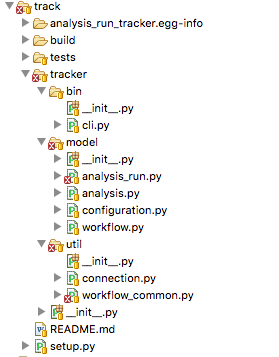
\includegraphics{tracker_module_files}
\centering
\caption {File hierarchy of the tracker module}
\label{fig:tracker_module_files}
\end{figure}

At the root of the hierarchy are the README file and the module installation script \mintinline{sh}{setup.py}. Inside the \mintinline{sh}{bin} directory is the Analysis Tracker CLI implementation - \mintinline{sh}{cli.py}. Inside the \mintinline{sh}{model} directory lies the implementation of the main model objects - Workflow, Analysis, Analysis Run, and Configuration. We describe the first three of these objects in detail in this section and the last one in Section \ref{sec:workflow_configuration_design}. Inside the \mintinline{sh}{util} directory are utility functions -  \mintinline{sh}{connection.py} for connecting to the Run Tracking Database, and  \mintinline{sh}{workflow_common.py} for implementations of common workflow tasks.

The overall model can be seen in Figure \ref{fig:analysis_tracker_model}

\begin{figure}[H]
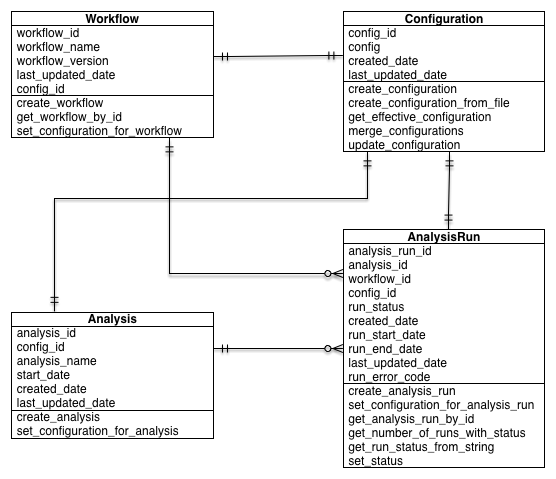
\includegraphics[width=\textwidth]{analysis_tracker_model}
\centering
\caption {UML model of the Analysis Tracker.}
\label{fig:analysis_tracker_model}
\end{figure}

\paragraph{The Workflow} object represents a workflow definition. Every workflow managed by Butler should have a corresponding Workflow object representing it. It has the following fields:

\begin{description}
\item [workflow\_id (UUID)] - This is the unique identifier of this workflow.
\item [workflow\_name (String)] - This is a human-friendly name for the workflow.
\item [workflow\_version (String)] - It is important to record what version of a workflow is being used, as updates are frequently made during the workflow lifecycle.
\item [last\_updated\_date (datetime)] - Timestamp of last update to this object.
\item [config\_id (UUID)] - The unique identifier of the corresponding Configuration object.
\end{description}

The Workflow object implements the following methods:

\begin{description}
\item [\mintinline{python}{create_workflow(workflow_name, workflow_version, config_id)}] - Create a new workflow object with given name, version, and configuration.
\item [\mintinline{python}{get_workflow_by_id(workflow_id)}] - Retrieve the workflow with ID \mintinline{python}{workflow_id} from persistent storage.
\item [\mintinline{python}{set_configuration_for_workflow(workflow_id, config_id)}] - Update the workflow configuration to configuration with ID \mintinline{python}{config_id}.
\end{description}

\paragraph{The Analysis} object represents a scientific analysis. It serves the purpose of aggregating the running of a set of workflows on a set of data samples together into a single unit of execution that can be referred to for organization purposes. The Analysis has the following fields.

\begin{description}
\item [analysis\_id (UUID)] - This is the unique identifier of this Analysis.
\item [analysis\_name (String)] - This is a human-friendly name for the Analysis.
\item [start\_date (datetime)] - Date of when the Analysis is meant to start.
\item [created\_date (datetime)] - Date of when the Analysis was created.
\item [last\_updated\_date (datetime)] - Timestamp of last update to this object.
\item [config\_id (UUID)] - The unique identifier of the corresponding Configuration object.
\end{description}

The Analysis object has the following methods:

\begin{description}
\item [\mintinline{python}{create_analysis(analysis_name, start_date, config_id)}] - Create a new Analysis object with given name, \mintinline{python}{start_date}, and configuration.
\item [\mintinline{python}{set_configuration_for_analysis(analysis_id, config_id)}] - Update the Analysis configuration to configuration with ID \mintinline{python}{config_id}.
\end{description}

\paragraph{The AnalysisRun} object represents the invocation of a particular Workflow on a particular Data Sample, within the scope of a particular Analysis. This object is central to the Analysis Tracking functionality. The AnalysisRun object has the following fields:

\begin{description}
\item [analysis\_run\_id (UUID)] - This is the unique identifier of this Analysis Run.
\item [analysis\_id (UUID)] - This is the unique identifier of the Analysis for this Analysis Run.
\item [workflow\_id (UUID)] - This is the unique identifier of the Workflow for this Analysis Run.
\item [run\_status (int)] - This integer field indicates the status of this Analysis Run. Status can be one of \mintinline[breaklines=true]{python}{RUN_STATUS_READY, RUN_STATUS_SCHEDULED, RUN_STATUS_IN_PROGRESS, RUN_STATUS_COMPLETED, RUN_STATUS_ERROR}.
\item [created\_date (datetime)] - Date of when the Analysis Run was created.
\item [run\_start\_date (datetime)] - Date of when the Analysis Run started.
\item [run\_end\_date (datetime)] - Date of when the Analysis Run ended.
\item [last\_updated\_date (datetime)] - Timestamp of last update to this object.
\item [run\_error\_code (int)] - Integer pointing to an error code of Runs that ended in error.
\item [config\_id (UUID)] - The unique identifier of the corresponding Configuration object.
\end{description}

The Analysis Run object implements the following methods:

\begin{description}
\item [\mintinline{python}{get_run_status_from_string(run_status_string)}] - Translate string-based run statuses into int-based ones.
\item [\mintinline{python}{create_analysis_run(analysis_id, config_id, workflow_id)}] - Create an AnalysisRun and store in the database.
\item [\mintinline{python}{set_configuration_for_analysis_run(analysis_run_id, config_id)}] - Update the AnalysisRun configuration to configuration with ID \mintinline{python}{config_id}.
\item [\mintinline{python}{get_analysis_run_by_id(analysis_run_id)}] - Get the Analysis Run with ID \mintinline{python}{analysis_run_id}.
\item [\mintinline{python}{set_ready(my_run)}] - Set the status of a given analysis run to \mintinline{python}{RUN_STATUS_READY}. Only possible if the current status is not \mintinline{python}{RUN_STATUS_IN_PROGRESS}.
\item [\mintinline{python}{set_scheduled(my_run)}] - Set the status of a given analysis run to \mintinline{python}{RUN_STATUS_SCHEDULED}. Only possible if the current status is \mintinline{python}{RUN_STATUS_READY}.
\item [\mintinline{python}{set_in_progress(my_run)}] - Set the status of a given analysis run to \mintinline{python}{RUN_STATUS_IN_PROGRESS}. Only possible if the current status is \mintinline{python}{RUN_STATUS_SCHEDULED}.
\item [\mintinline{python}{set_completed(my_run)}] - Set the status of a given analysis run to \mintinline{python}{RUN_STATUS_COMPLETED}. Only possible if the current status is \mintinline{python}{RUN_STATUS_IN_PROGRESS}.
\item [\mintinline{python}{set_error(my_run)}] - Set the status of a given analysis run to \mintinline{python}{RUN_STATUS_ERROR}.
\item [\mintinline{python}{get_number_of_runs_with_status(analysis_id, run_status)}] - Returns the number of AnalysisRuns of a given status.
\end{description}

As can be seen from the description of the methods of \mintinline{python}{AnalysisRun} these objects follow a particular lifecycle that is represented by their \mintinline{python}{status} attribute. The rules that govern allowable status transitions are encoded within the series of \mintinline{python}{set_*} methods and are summarized in Figure \ref{fig:analysis_run_status_transitions}

\begin{figure}[H]
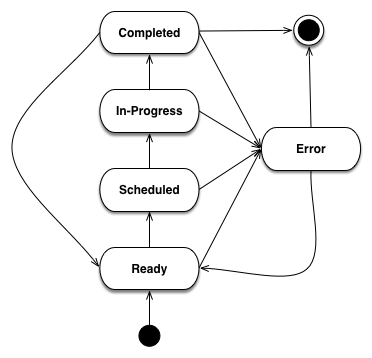
\includegraphics{analysis_run_status_transitions}
\centering
\caption {State Diagram of Analysis Run Status Transitions.}
\label{fig:analysis_run_status_transitions}
\end{figure}

When an \mintinline{python}{AnalysisRun} is first created it does not have a status. Once the object is fully initialized it is given a Ready status, indicating that it is ready to be scheduled for execution. Once the Scheduler has scheduled the Run for execution it is given a Scheduled status. When workflow execution starts the Run is marked In-Progress. Once the Run is successfully completed it enters a Completed status. If, at any point, the Run encounters an error condition it cannot recover from, the Run Status is set to Error. When the error condition is addressed the Run status should be set to Ready so that it can start from the beginning.

\paragraph{The workflow\_common.py} file within the tracker module contains a number of convenience functions that workflows can use to perform common tasks. Currently the following functions are supported:

\begin{description}
\item [\mintinline{python}{get_config(kwargs)}] - Get the Configuration supplied to this Workflow.
\item [\mintinline{python}{get_sample(kwargs)}] - Get the sample assigned to this Workflow.
\item [\mintinline{python}{start_analysis_run(**kwargs)}] - Mark the Analysis Run of this Workflow In-Progress.
\item [\mintinline{python}{complete_analysis_run(**kwargs)}] - Mark the Analysis Run of this Workflow Complete. 
\item [\mintinline{python}{set_error_analysis_run(**kwargs)}] - Mark the Analysis Run of this Workflow as Error.
\item [\mintinline{python}{validate_sample(**kwargs)}] - Test whether the sample files are accessible to the workflow.
\item [\mintinline{python}{call_command(command, command_name, cwd=None)}] - Wrapper around Python's \mintinline{python}{subprocess.call} method that captures logging information.
\item [\mintinline{python}{compress_sample(result_filename, config)}] - Compress the sample with gzip.
\item [\mintinline{python}{uncompress_gzip_sample(result_filename, config)}] - Uncompress the sample.
\end{description}

Every workflow should begin by starting the corresponding Analysis Run, and finish by completing it to ensure appropriate tracking of information throughout the system.

\paragraph{The connection.py} file is also a key component of the tracker module because it provides a means to communicate with the Run Tracking Database.

The Run Tracking Database is a PostgreSQL database this is set up to persist all of the Analysis related information into permanent storage in order to fulfill the System of Record requirements of Section \ref{sec:system_of_record}. Specifically, the Run Tracking Database contains a relational model that corresponds to the Python objects described above. These tables are as follows:

\begin{table}[H]
\renewcommand{\arraystretch}{1.2} 
\centering
\begin{tabular}{@{}lll@{}}
\toprule
Column Name & Type & Constraint\\
\midrule
workflow\_id & serial & PRIMARY KEY\\
config\_id & uuid & REFERENCES configuration(config\_id)\\
workflow\_name & varchar(255) & \\
workflow\_version & varchar(255) & \\
created\_date & timestamp\\
last\_updated\_date & timestamp\\
\bottomrule
\end{tabular}
\caption{Database table workflow}
\end{table}

\begin{table}[H]
\renewcommand{\arraystretch}{1.2} 
\centering
\begin{tabular}{@{}lll@{}}
\toprule
Column Name & Type & Constraint\\
\midrule
analysis\_id & serial & PRIMARY KEY\\
config\_id & uuid & REFERENCES configuration(config\_id)\\
analysis\_name & varchar(255) & \\
start\_date & timestamp & \\
created\_date & timestamp\\
last\_updated\_date & timestamp\\
\bottomrule
\end{tabular}
\caption{Database table analysis}
\end{table}

\begin{table}[H]
\renewcommand{\arraystretch}{1.2} 
\centering
\begin{tabular}{@{}lll@{}}
\toprule
Column Name & Type & Constraint\\
\midrule
analysis\_run\_id & serial & PRIMARY KEY\\
analysis\_id & serial & REFERENCES analysis(analysis\_id)\\
workflow\_id & serial & REFERENCES workflow(workflow\_id)\\
config\_id & uuid & REFERENCES configuration(config\_id)\\
run\_status & integer & NOT NULL\\
created\_date & timestamp\\
run\_start\_date & timestamp\\
run\_end\_date & timestamp\\
last\_updated\_date & timestamp\\
run\_error\_code & integer\\
\bottomrule
\end{tabular}
\caption{Database table analysis\_run}
\end{table}

In order to maintain a mapping between the Python objects in the tracker module and the tables in the Run Tracking Database as well as to avoid getting tied to a particular SQL dialect we utilize the SQL Alchemy Object Relational Framework. This framework allows us to avoid an explicit mapping between table columns, and object fields. Instead, SQL Alchemy is able to introspect the relational schema and add the object fields as necessary that correspond to the columns. Furthermore, updates to the Python objects are automatically translated to SQL \mintinline{sql}{UPDATE} statements and executed as necessary. This framework allows us to change to a different SQL Engine if necessary, without having to change most of the code.

\subsection{Workflow Configuration} 
\label{sec:workflow_configuration_design}

In order to fulfill the workflow configuration and parametrization requirements described in the Analysis Configuration sub-section of Section \ref{sec:workflow_definitions} Butler implements a tri-level configuration mechanism, allowing the user to specify configurations at Workflow, Analysis, and Analysis Run levels. At runtime all three configuration levels are merged into one \emph{effective} configuration that applies within the execution context.

\begin{figure}[H]
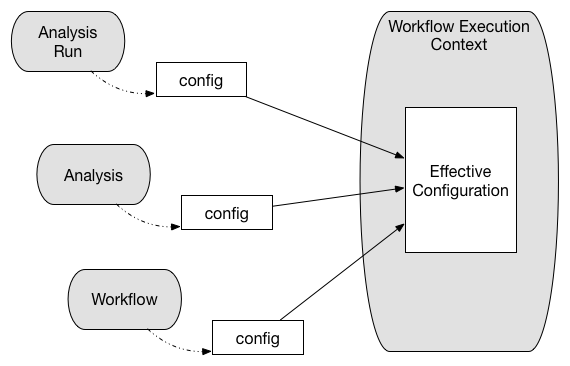
\includegraphics[width=\textwidth]{effective_configuration}
\centering
\caption {Tri-level configuration combines into an effective configuration at runtime.}
\label{fig:effective_configuration}
\end{figure}

The configuration facility is built into the \mintinline{python}{tracker} module, and is backed by a Run Tracking Database configuration table for persistence.

Because it is important for configuration to be both human-readable and machine-readable Butler uses the JSON format to encode configuration information. PostgreSQL, in turn, has native support for storage and deep querying of JSON values, thus making it an ideal choice for configuration persistence.

\subsubsection {Configuration Mechanism}

The mechanism by which configuration works is as follows:

A workflow author provides, together with their workflow definition, a JSON file that contains the most coarse-grained configurations related to the workflow. A system operator may customize some of these values before adding the workflow to a deployed version of Butler. Once the workflow is added to the system its accompanying configuration is persisted to the database.

A user who is running an analysis defines an analysis-level JSON file with more fine-grained configuration values. Algorithm parameters and flags are typical such values that vary from one analysis to the next. These are also persisted to the database along with the analysis definition.

As the analysis run corresponds to running a particular workflow in the context of a particular analysis on a particular sample, the user needs to generate a separate JSON configuration file for each sample in the analysis. These files will contain the most fine-grained configurations. Typical values at this level indicate where to locate the particular sample file for this run, and where to store the run results. An effective way to generate many JSON files for these runs is via a script.

When a workflow is executed on a particular sample, the JSON files corresponding to all three levels of configuration are retrieved from the database, merged, and parsed into a Python dictionary. This dictionary is then made available within the workflow execution context to guide workflow decision logic.

\subsection{Workflow Runtime Management}

Workflow Runtime Management encompasses the tools that are available to the user for the purpose of managing workflow execution. In Butler there are three separate mechanisms that exist for this purpose. These are:

\begin{itemize}
\item Butler CLI
\item Airflow CLI
\item Airflow Web UI
\end{itemize}

\subsubsection{Butler CLI}

The Butler CLI allows the user to create the various analysis management objects described in Section \ref{sec:analysis_tracker} via a Command Line Interface. The following commands are supported:

\paragraph{\mintinline{shell}{create-workflow}} - creates a new workflow and supports the following parameters:
\begin{description}
\item [-n, -\--workflow\_name] - The name of the workflow.
\item [-v, -\--workfow\_version] - The version of the workflow.
\item [-c, -\--config\_file\_location] - Path to the workflow configuration JSON file.
\end{description}

\paragraph{\mintinline{shell}{create-analysis}} - creates a new analysis and supports the following parameters:
\begin{description}
\item [-n, -\--analysis\_name] - The name of the analysis.
\item [-d, -\--analysis\_start\_date] - The starting date of the analysis.
\item [-c, -\--config\_file\_location] - Path to the analysis configuration JSON file.
\end{description}

\paragraph{\mintinline{shell}{launch-workflow}} - launches workflow execution and supports the following parameters:

\begin{description}
\item [-w, -\--workflow\_id] - ID of the workflow to launch.
\item [-a, -\--analysis\_id] - ID of the analysis to launch the workflow under.
\item [-c, -\--config\_location] - Path to a directory that contains analysis run configuration JSON files that will be launched. 
\end{description}

\paragraph{\mintinline{shell}{update-config}} - Update the configuration for a workflow or analysis.

\begin{description}
\item [-w, -\--workflow\_id] - ID of the workflow to update.
\item [-a, -\--analysis\_id] - ID of the analysis to update.
\item [-c, -\--config\_file\_location] - Path to the new config file.
\end{description}

\paragraph{\mintinline{shell}{get-run-count}} - Print to stdout the number of analysis runs for a particular analysis.

\begin{description}
\item [-a, -\--analysis\_id] - ID of the analysis to look up.
\item [-s, -\--run\_status] - Restrict the lookup to runs with a particular status
\end{description}

\subsubsection{Airflow CLI}

The Airflow CLI is part of the generic Airflow framework and provides a number of commands for workflow management. We describe several of the most useful ones below:

\paragraph{\mintinline{shell}{airflow}} - The main Airflow CLI command, with these supported sub-commands:

\begin{description}
\item [webserver] - Start an instance of the Airflow Web UI.
\item [scheduler] - Start an instance of the Airflow Scheduler.
\item [worker] - Start an instance of the Airflow Worker.
\item [flower] - Start an instance of the Airflow Flower, which is a monitoring tool.
\item [clear] - Clear the state of tasks that have failed or are stuck to allow them to be scheduled again.
\item [task\_state] - Print out the state of a task.
\item [initdb] - Initialize an empty Airflow database.
\item [resetdb] - Reset an Airflow database to the empty state.
\item [list\_dags] - List all of the available workflows.
\item [list\_tasks] - List all of the tasks for a particular workflow.
\end{description}

Butler provides wrappers for the \mintinline{shell}{webserver, scheduler, worker, and flower} commands so that they can be run as system services.

\subsubsection{Airflow Web UI}

The Airflow Web UI provides an interactive dashboard that allows the user to monitor the progress of workflows and workflow tasks, as well as taking some remedial actions when tasks run into trouble.

\begin{figure}[h]
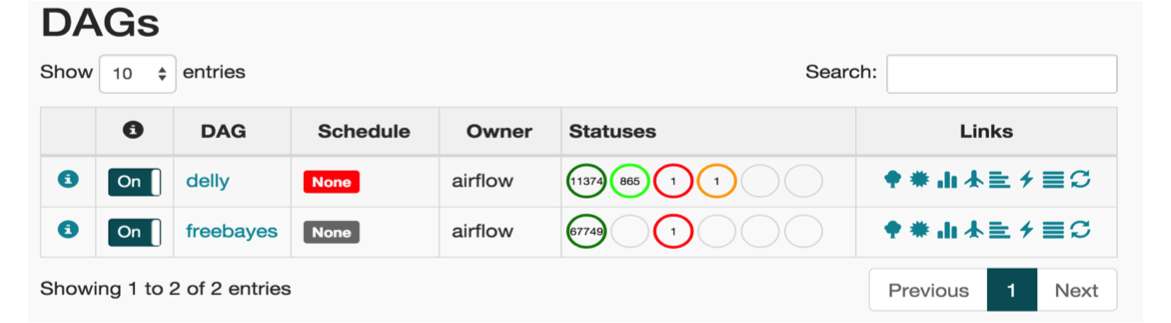
\includegraphics[width=\textwidth]{airflow_web_ui_main_page}
\centering
\caption {The main page of the Airflow Web UI}
\label{fig:airflow_web_ui_main_page}
\end{figure}

The main page of the Web UI features a listing of the available workflows, along with the breakdown of workflow tasks by status. In Figure \ref{fig:airflow_web_ui_main_page} we see two workflows - freebayes and delly. The delly workflow has 11374 completed tasks, 865 in-progress tasks, 1 failed task, and 1 task with a failed ancestor. The user can click on any of the task statuses to navigate to a task listing page that gives a comprehensive list of tasks along with their key attributes (see Figure \ref{fig:airflow_task_instances}.

\begin{figure}[h]
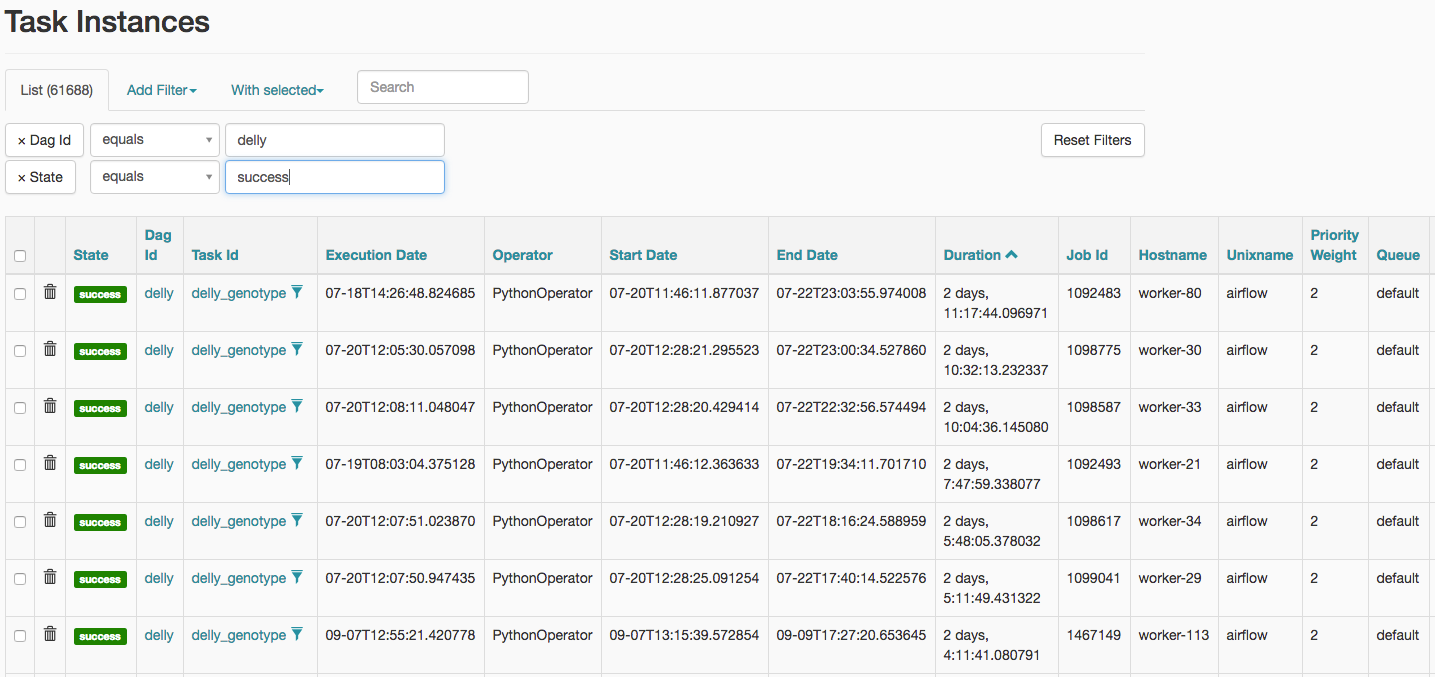
\includegraphics[width=\textwidth]{airflow_task_instances}
\centering
\caption {Listing of task instances for the freebayes workflow with status of "success".}
\label{fig:airflow_task_instances}
\end{figure}

Clicking on one of the task instances will bring up a graphical view of the workflow the task belongs to and allow the user to further investigate that workflow's execution (see Figure \ref{fig:airflow_workflow_details}). This view shows the status of all tasks in the corresponding workflow instance as well as providing links to various reports.

\begin{figure}[h]
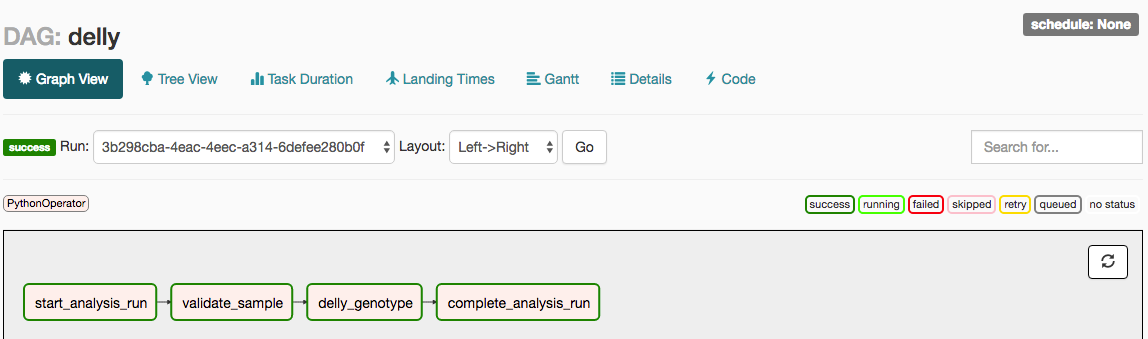
\includegraphics[width=\textwidth]{airflow_workflow_details}
\centering
\caption {Details of the execution of a delly workflow with ID 3b298cba-4eac-4eec-a314-6defee280b0f.}
\label{fig:airflow_workflow_details}
\end{figure}

When the user clicks on a particular task instance within the workflow execution a popup window allows them to take a number of actions, such as forcing the task to be run immediately, clearing the task state (for failed tasks) so that it can be run again, or marking the task as successfully completed (possibly with all upstream and downstream tasks). These options are depicted in Figure \ref{fig:airflow_task_actions}

\begin{figure}[h]
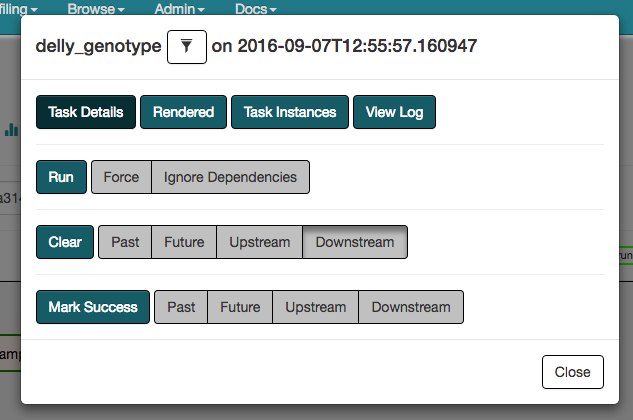
\includegraphics[scale=0.3]{airflow_task_actions}
\centering
\caption {A list of actions that can be taken on a workflow task via the Web UI.}
\label{fig:airflow_task_actions}
\end{figure}

\section{Operational Management}\label{sec:operational_management}

Managing large fleets of Virtual Machines as they perform data analysis at scale across multiple cloud computing environments is a major challenge due to the sheer number of possible scenarios that could lead to the system crashing, stalling, or otherwise falling out of control, with the negative impact on the end user in terms of project costs and timeline increasing with the scale of the computation being undertaken. The tools available to the user to detect and deal with these issues thus form a key component of a comprehensive analysis framework and set Butler apart from other frameworks in this space.

In general, the Operational Management tools fall into two categories, those that collect observations about the state of each component in the system at runtime, and those that aggregate this data and present it to the user in the form of queryable databases and management reports. Furthermore, as specified in the requirements of Section \ref{sec:troubleshooting} we delineate two major sources of data that is indicative of system state - System Metrics, and Server Logs. While metrics provide more of a coarse-grained view of the overall health of a particular Virtual Machine, server logs can give much more of a fine-grained view of the underlying system at an application level, and down to individual lines of code that are running at any given time. Butler has dedicated components for the collection and management of these data sets and we describe these next.

\begin{figure}[h]
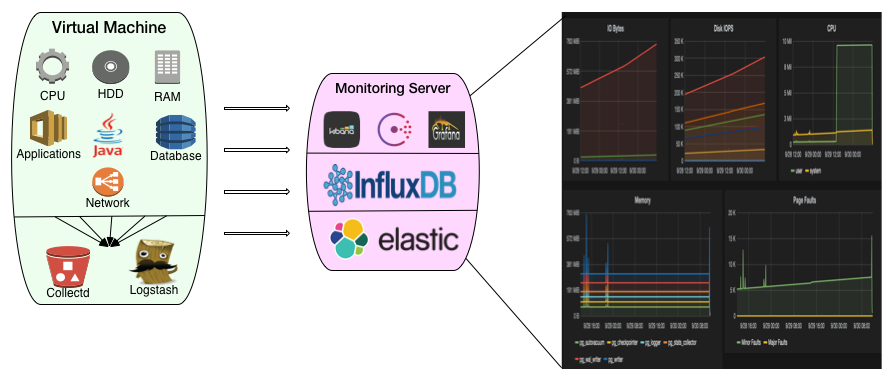
\includegraphics[width=\textwidth]{monitoring_server}
\centering
\caption {Metric monitoring system components}
\label{fig:monitoring_server}
\end{figure}

\subsection{Monitoring Metric Collection}

The overall health of any VM in a cloud computing cluster can be evaluated and ascertained with respect to a set of key metrics that are observable at runtime. Some metrics are general enough that they apply to all Virtual Machines, these include measurements of CPU utilization, RAM, Disk, and Network usage. Other metrics are more specific to the role that the VM is playing within the cluster. A Database Server will benefit from having the number of open DB connections, transaction rate, rollback rate, and average query runtime monitored. Other entities such as Web Servers and Queues have their own unique metrics of interest.

Each VM runs a metric collection daemon called \mintinline{shell}{collectd} which is an Open Source package that is able to make periodic measurements of a large number of system metrics and ship them off to a centralized Metrics Store. The definition for which metrics are collected is specified in a special configuration file. An example of such configuration is demonstrated in Listing \ref{lst:collectd_config}. This listing provides examples of the setup for generic metrics like CPU, and memory, as well as for more special metrics, like those collected for PostgreSQL databases.

Because we are interested in observing not only the metrics as they are measured in the present, but also the dynamics of how metric values change over time, we need a mechanism for persisting the metrics values. For this purpose the Monitoring Server component of Butler ships with an instance of a database product called InfluxDB\autocite{InfluxDB} which is an Open Source database system that is optimized for recording time series data. The configuration for the \mintinline{shell}{network} plugin in Listing \ref{lst:collectd_config} demonstrates how InfluxDB server URL is provided to CollectD to enable metrics persistence in this centralized data store.

InfluxDB is a scalable database system that can operate in a distributed manner as a Raft\autocite{ongaro2014search} cluster. Data is written into shards based on a data retention policy. The underlying engine stores the data as a Time-Structured Merge Tree (TSM) which is a customization of the Log-Structured Merge-Tree\autocite{o1996log} data structure. To the end user the data is organized as a collection of \mintinline{shell}{points}. Each point has a \mintinline{shell}{timestamp}, belongs to a \mintinline{shell}{measurement}, and records a set of \mintinline{shell}{tag_values} that correspond to a set of \mintinline{shell}{tag_keys}. A particular \mintinline{shell}{measurement} coupled with a retention policy then forms a \mintinline{shell}{series}.

As an example, when tracking RAM, our \mintinline{shell}{measurement} is called \mintinline{shell}{memory_value}. The set of \mintinline{shell}{tag_keys} is:

\begin{itemize}
\item host
\item type
\item type\_instance
\end{itemize}

An example set of \mintinline{shell}{tag_values} might be:

\begin{itemize}
\item worker-145
\item memory
\item free
\end{itemize}

The actual \mintinline{shell}{points} corresponding to this combination of \mintinline{shell}{tag_values} and collected over the period of 1 minute might look as follows:

\begin{figure}[h]
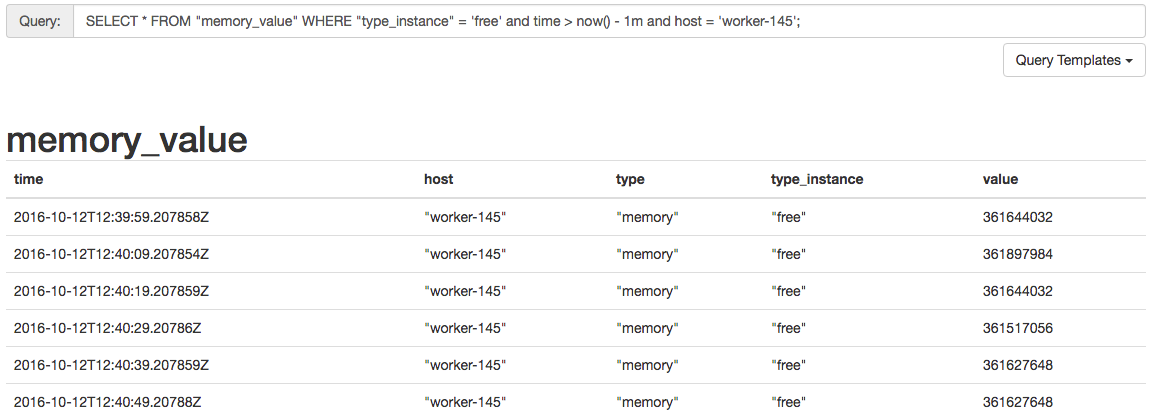
\includegraphics[width=\textwidth]{influxdb_example_query}
\centering
\caption {InfluxDB query results showing free memory on host worker-145 collected in a 1 minute time window.}
\label{fig:influxdb_example_query}
\end{figure}

As can be seen in Figure \ref{fig:influxdb_example_query}, data is queried via an SQL-like dialect which is accessible via a Web UI or via a REST\autocite[Chapter~5]{fielding2000architectural} API.

InfluxDB supports direct ingestion of collectd metrics data via a collectd connector which is configured in the InfluxDB configuration file.

\captionof{listing} {InfluxDB collectd connector configiuration. \label{lst:influxdb_config}}
\begin{minted}
[
breaklines=true,
linenos,
fontsize=\footnotesize,
frame=lines,
framesep=2mm,
baselinestretch=1.2
]
{yaml} 
[collectd]
  enabled = true
  bind-address = ":8096"
  database = "metrics"
  retention-policy = ""
  batch-size = 5000
  batch-pending = 10
  batch-timeout = "10s"
  read-buffer = 0
  typesdb = "/usr/share/collectd/types.db"
\end{minted}

\subsection{Monitoring Visualization}

The metrics collection system is collecting 50 different metrics per host on average, sampled at intervals of 10 seconds. Given a cluster of 200 Virtual Machines the monitoring system collects and stores 86,400,000 data points in a 24 hour time period. This volume of data is quite difficult for the user to comprehend and make use of, and Butler provides visualization tools to enable the display of aggregate statistics based on the monitoring data using a Graphical User Interface. The main goal of the visualizations is to give the user an overview of the trends observed within the compute cluster with respect to a set of representative performance metrics, and to alert the user to any conditions that threaten the health of Virtual Machines and the scientific analyses they run.

Visualization of performance metrics data is accomplished in Butler using an Open Source framework called Grafana\autocite{Grafana.net}. This framework provides a Web Interface that is able to connect to an instance of an InfluxDB database, issue queries and render the query results as dashboard of various graph styles, including line graphs, bar graphs, pie charts, and others. Reports generated by Grafana support parametrization of values as well as drill-through.

Butler ships with a number of pre-built reports and supports the addition of custom reports if necessary.

In general, Grafana is a website that the user logs onto to either author or view reports. When authoring reports the user needs to define a Data Source to connect the reports with data. In the case of Butler, the Data Source is connecting to the InfluxDB metrics database using the InfluxDB REST API.

\begin{figure}[h]
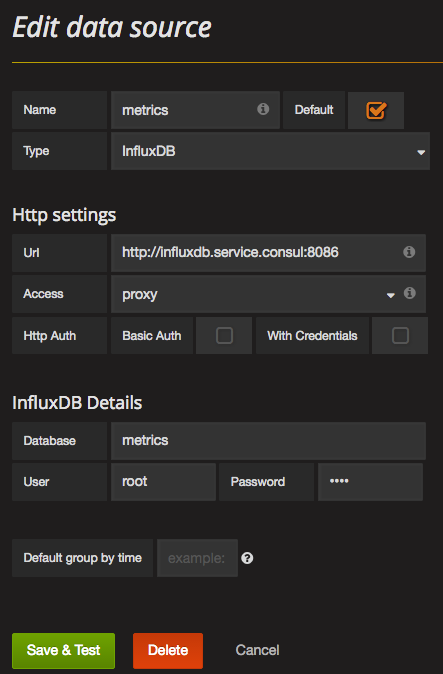
\includegraphics[scale=0.4]{grafana_data_source}
\centering
\caption {InfluxDB Data Source creation for Grafana.}
\label{fig:grafana_data_source}
\end{figure}

Once a connection to the Data Source is established the user can begin building dashboards. Dashboards are generally laid out in a grid-like fashion as a series of panels that are arranged into rows and columns. Each panel contains a graph. Data is fed into the graph by means of an InfluxDB Query Language query, possibly with additional parameters specified by the report.  In addition to the query itself, the user can customize the axes, legend, and other attributes of each graph. Once the report is ready it can be exported into a JSON format and checked into a source code repository so that it can persist if the VM hosting the Grafana instance needs to be recreated.

\begin{figure}[h]
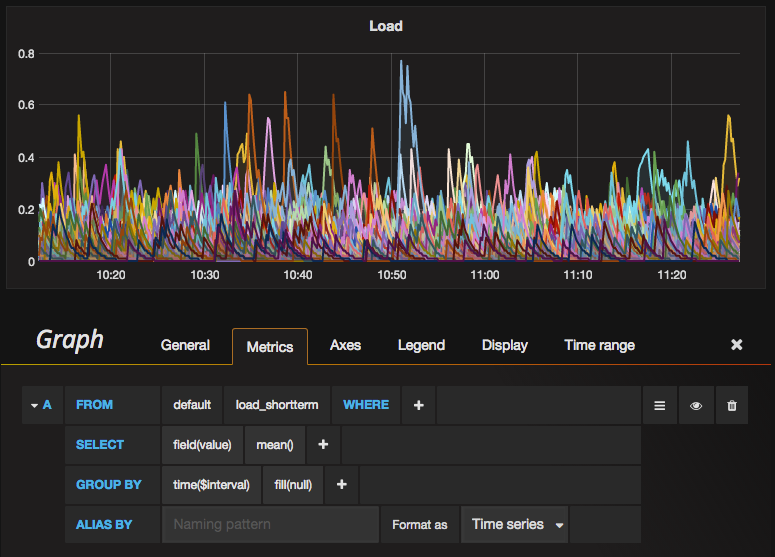
\includegraphics[width=\textwidth]{grafana_report_editing}
\centering
\caption {Editing a Grafana dashboard panel.}
\label{fig:grafana_report_editing}
\end{figure}

Butler comes with a set of basic dashboards defined out-of-the-box that will aid the user in monitoring of overall system health. The most important dasbhoards are:

\begin{description}
\item [Cluster Overview] - Gives a high level overview of the health of the entire cluster, tracking metrics such as load (blended health metric), CPU utilization, Memory, Disk IOPS, Network Packet Rate, Disk Read/Write Rates, and Disk Space
\item [Salt Master] - Detailed monitoring of the Salt Master VM, including CPU, Memory, Network Packet Rate, Disk Read/Write Rates, Disk IOPS, and Disk Space.
\item [Database Server] - Detailed monitoring of the Database Server VM, including DB-specific metrics such as - DB Connections, Number of Transactions, Number of Queries, Number of Query Plans, Number of Rows, DB Size on Disk, as well as the general VM health metrics.
\end{description}

\begin{figure}[h]
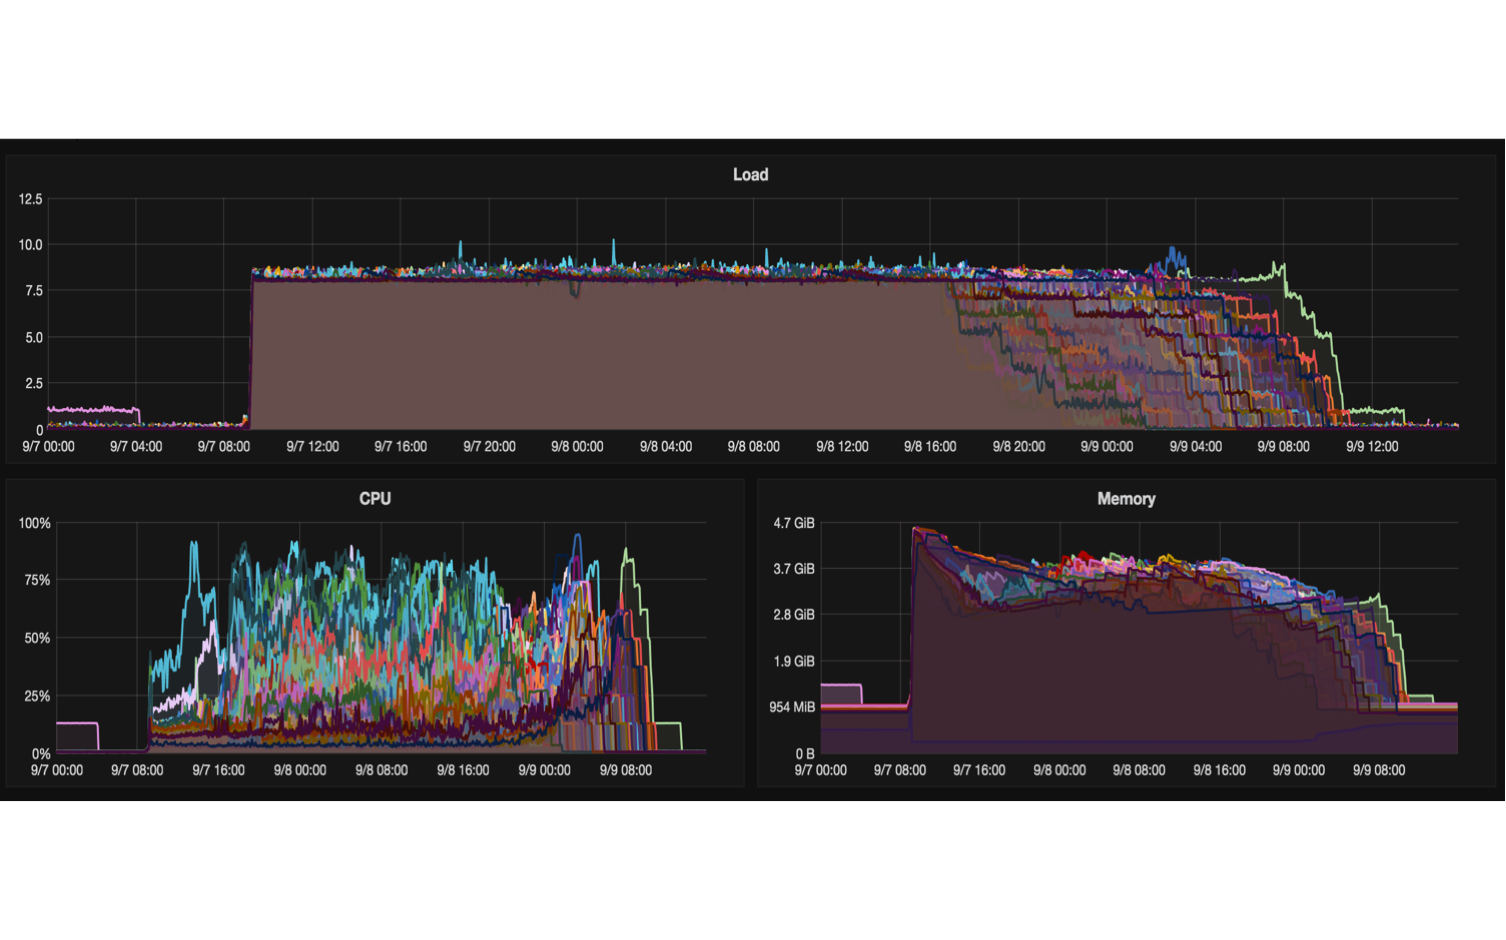
\includegraphics[width=\textwidth]{grafana_cluster_overview_normal}
\centering
\caption {Cluster Overview dashboard during normal operation.}
\label{fig:grafana_cluster_overview_normal}
\end{figure}

In practice the Cluster Overview dashboard is the most consistently useful report because it provides an at-a-glance view of the health of the entire cluster. Figure \ref{fig:grafana_cluster_overview_normal} demonstrates a typical scenario of cluster usage during normal operation. It is evident that the cluster starts off without any appreciable load, once a set of workflows is scheduled system load increases across the entire cluster and remain stable until, towards the end of the execution, machines start running out of work, and load of the system gradually decreases. Throughout the execution the memory profile is relatively stable and consistent across the machines in the cluster. Although the CPU profile appears spiky, this is the natural CPU utilization profile for the particular set of workflows that were executing at the time the image was captured.

\begin{figure}[h]
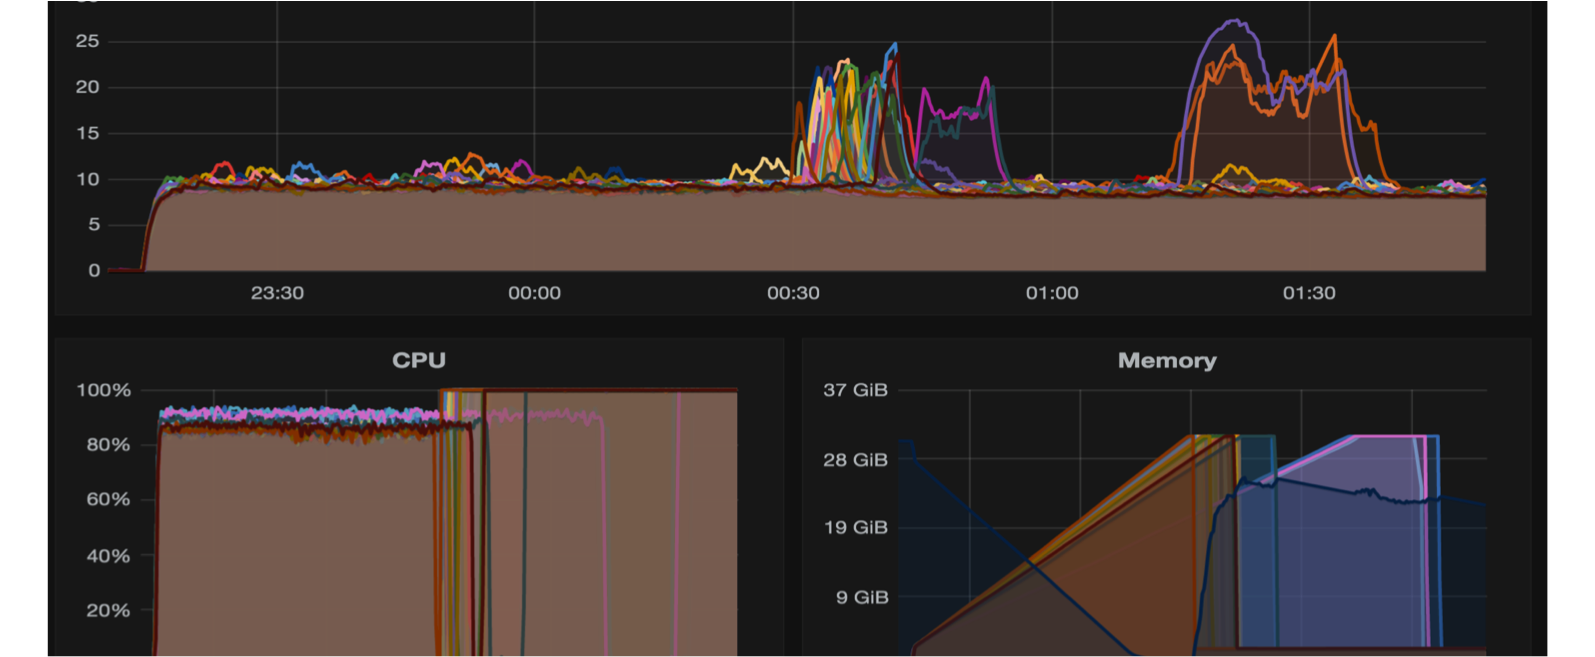
\includegraphics[width=\textwidth]{grafana_cluster_overview_issue}
\centering
\caption {Cluster Overview dashboard demonstrating a cluster-wide issue.}
\label{fig:grafana_cluster_overview_issue}
\end{figure} 

Figure \ref{fig:grafana_cluster_overview_issue}, on the other hand, demonstrates an example of how a cluster-wide issue can be identified via the Cluster Overview dashboard. Here we see a similar profile at the beginning of workflow execution, where the jobs get kicked off and load is stable, but at around 00:30 we start seeing uncharacteristic spikes in system load, with sporadic doubling of load metric values. Furthermore, the CPU utilization appears to drop to 0 at the same time, and the memory profile is highly irregular. This pattern signifies to the user that an issue is affecting the cluster during this particular time, and further investigation is needed. With that knowledge, the user can use other reports to try to pinpoint the source of the issue, or it may be necessary to directly log on to the affected VM hosts to investigate further.

Because collectd allows collecting metrics from a particular named process, and because Grafana allows the creation of new dashboards on the fly, it is common and convenient for the user to develop a set of custom dashboards that are targeted towards the specific workflows that they are running, thus providing much more fine-grained visibility into the runtime behaviour of the system. Together with the built in reports these custom dashboards provide a powerful and flexible set of capabilities for successful operational management of the Butler system. 

\subsection{Server Log Collection and Visualization} 
\label{sec:design_log_collection}

Almost every application that runs on a computer is generating some sort of log file. On Unix-based environments most system-level applications will write to a common log known as syslog. But many other applications will write their own custom logs to their own specific locations. Messages written to a log file typically run the gamut from INFO statements that mark the normal operation of an application, all the way to ERROR which signify error conditions. Thus, a log file, potentially provides a wealth of information about both normal operation and system issues as they occur, and is typically one of the most reliable sources for information on application crashes. On the other hand, when operating a complex distributed system, such as a large scale workflow execution framework which runs on hundreds of Virtual Machines, the number and size of logs can become overwhelming to the point of ceasing to remain useful.  

Because of the potentially extremely high value of the information contained in server logs, we deploy a system of log harvesting and centralized storage that enables the Virtual Machines that are part of Butler to parse the logs that are being generated locally for interesting events, and send those events to a centralized search index which is amenable to efficient querying and visualization. Although the three tools that we use to solve the centralized logging problem have been developed independently, they have since been acquired by a single company Elasticsearch BV. These three tools form what is known as the ELK stack - Elasticsearch\autocite{Elasticsearch}, Logstash\autocite{Logstash}, and Kibana\autocite{Kibana}.

Each Virtual Machine in the cluster runs a log shipper - Filebeat. It is responsible for finding, harvesting, and locally aggregating logs.

\begin{figure}[h]
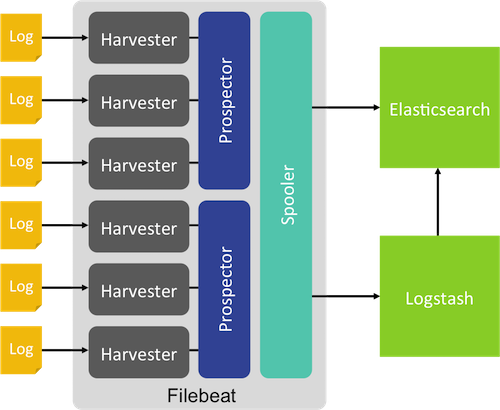
\includegraphics[scale=1]{filebeat}
\centering
\caption {Filebeat Architecture (taken from https://www.elastic.co).}
\label{fig:filebeat}
\end{figure}

As shown in Figure \ref{fig:filebeat}, Filebeat consits of a set of Prospectors (see Listing \ref{lst:filebeat_prospectors})which monitor and search log directories specified in the Filebeat configuration file. Corresponding to each log file that is found by Prospectors a separate Harvester is started which is responsible for ingesting the log file and sending the information to a Spooler. The Spooler aggregates information sent from Harvesters and forwards it onto Logstash for further parsing.

Logstash runs on a separate centralized server and is responsible for parsing the logs forwarded from Filebeat and sending the parsed information on to the Elasticsearch index. The parsing is accomplished via 3 plugins - Input Plugin, Filter Plugin, and Output Plugin (see Figure \ref{fig:logstash_pipeline}). All three plugins are configured via the logstash configuration file.

\begin{figure}[h]
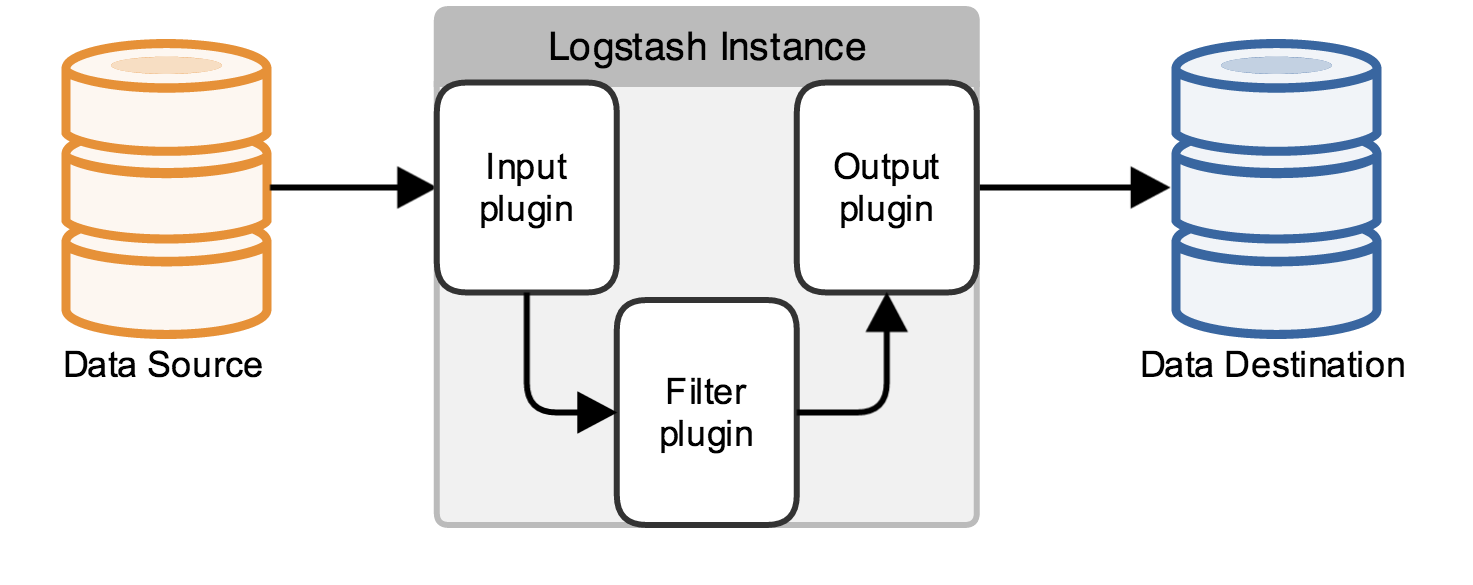
\includegraphics[scale=0.2]{logstash_pipeline}
\centering
\caption {A Logstash processing pipeline (taken from https://www.elastic.co).}
\label{fig:logstash_pipeline}
\end{figure}

The Input Plugin specifies where to listen to input data from. In the case of Butler we are expecting data to arrive in Filebeat format on port 5044.

The Filter plugin specifies how to parse the log file i.e. which messages from each type of log file we are interested in. The interesting messages are identified using a series of regular expressions known as grok patterns. 

The output plugin then specifies how to pass the filtered messages on to the Elasticsearch engine for indexing.

Elasticsearch is a general purpose scalable text indexing and search engine that supports clustering and sharding of data. Given its longterm use as a storage engine for log data and its scalability it is a great fit for Butler's log storage needs. Elasticsearch works by storing JSON formatted documents (in this case log messages) into an searchable index. 

Just as it is difficult to grasp and analyze performance metrics due to the number of data-points generated, it is as difficult to grasp log messages from a large cluster. We utilize a similar set of visualization tools to the ones we used for metrics, to solve this problem for server logs within Butler. The Kibana dashboarding framework allows us to create graphical dashboards that visualize log events of interest, as well as providing a web-based query interface to the Elasticsearch log messages index. Figure \ref{fig:kibana_pgsql_dashboard} shows a dashboard used in Butler for monitoring the Database Server.

\begin{figure}[h]
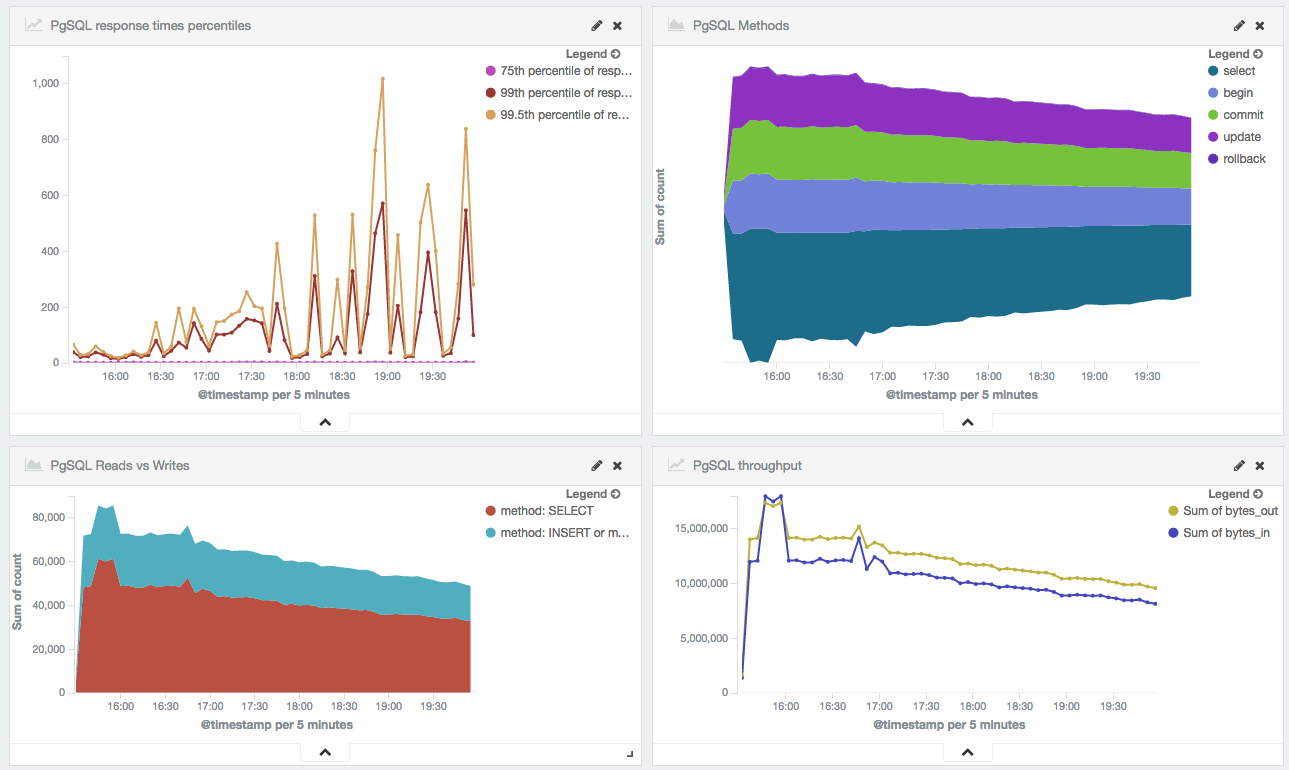
\includegraphics[width=\textwidth]{kibana_pgsql_dashboard}
\centering
\caption {Kibana dashboard for PostgreSQL monitoring.}
\label{fig:kibana_pgsql_dashboard}
\end{figure}
 
\subsection{Service Discovery} 
\label{sec:design_consul}

The Butler framework consists of many different services that reside on a number of different servers and need to be able to communicate with each other. To accomplish this in a flexible manner we need to establish a Service Registry so that IP addresses of servers that host particular services can be looked up by service name. To accomplish this Butler uses an Open Source service discovery framework called Consul\autocite{Consul_by_HashiCorp}.

Consul provides a cross-data-center distributed Service Name Registry that is available via HTTP and DNS protocols. In addition to registry capabilities Consul provides basic health checks for the underlying services, testing whether the IP and port the service is supposed to be listening on are actually reachable.

\begin{figure}[h]
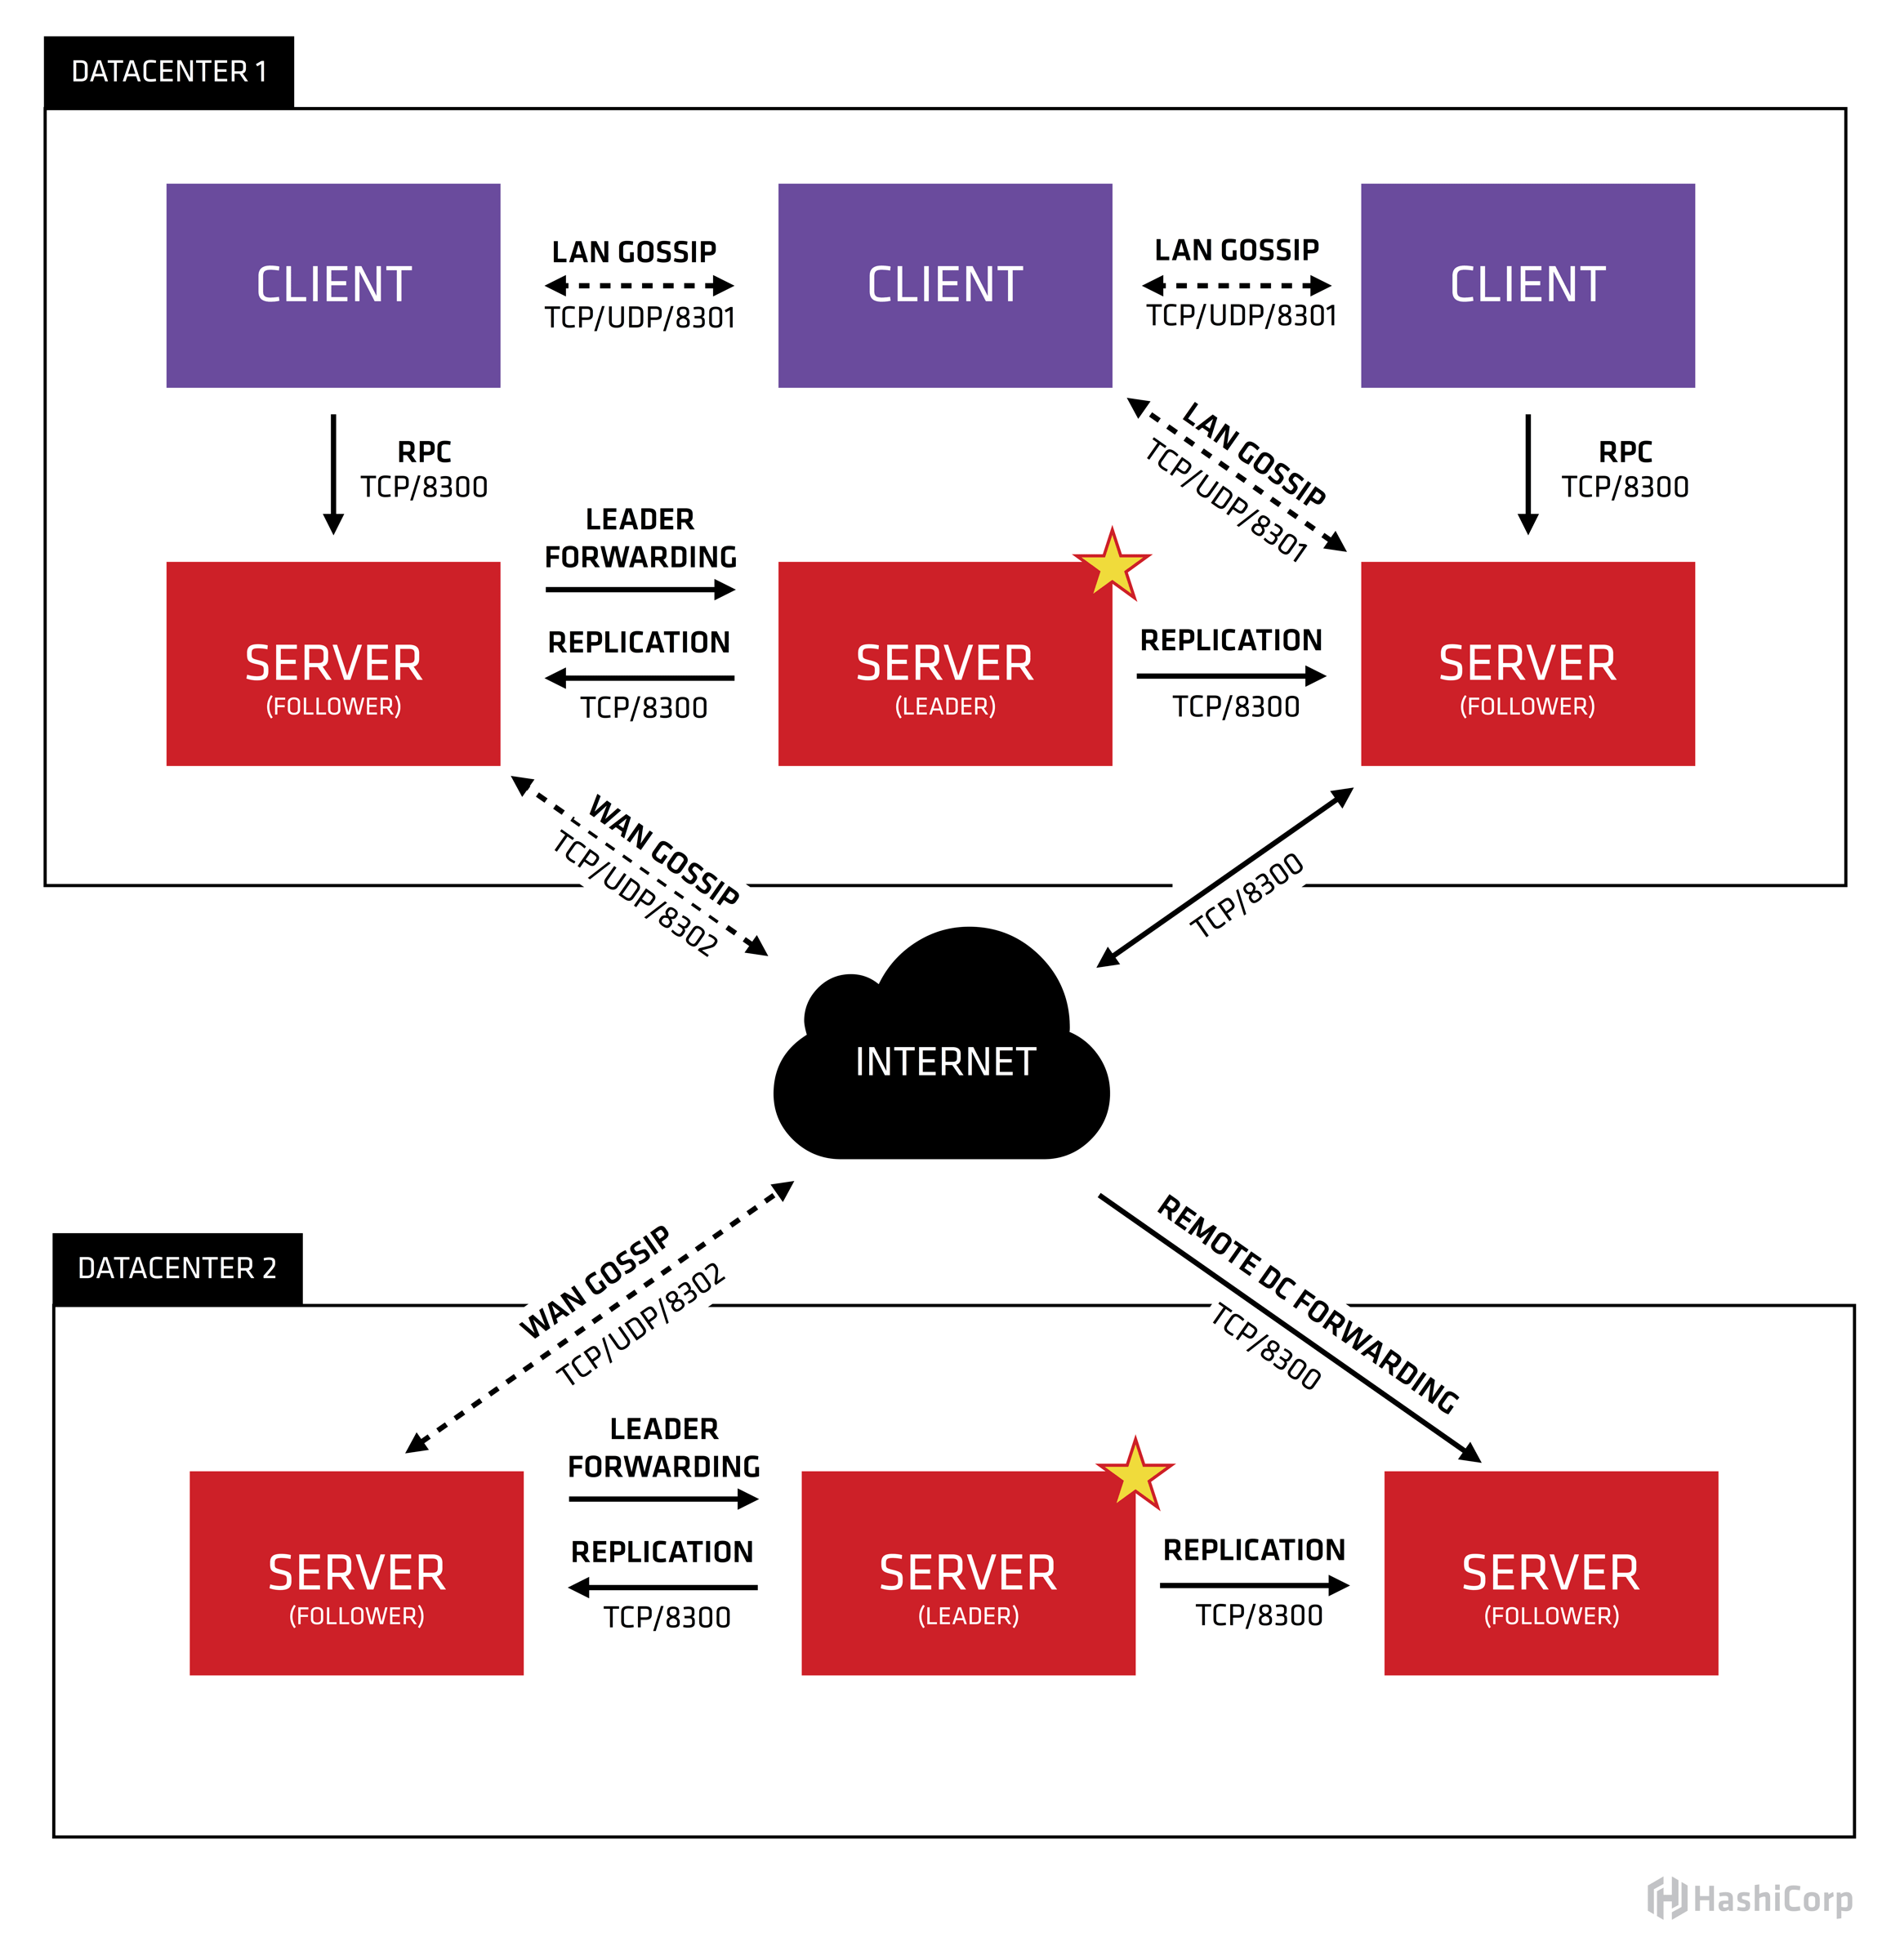
\includegraphics[scale=0.1]{consul_architecture}
\centering
\caption {Consul high level architecture (from \url{https://www.consul.io/docs/internals/architecture.html)}.}
\label{fig:consul_architecture}
\end{figure} 

Each VM in the cluster runs a Consul Agent which can be run in Server and Client modes. The set of Consul Servers form a Raft cluster and provide consensus-based responses to service lookup requests from clients. When new VMs are started they need to join the Consul cluster in order to be able to perform lookups, doing so requires knowing the IP address of at least one server. In Butler we use Saltstack's configuration capabilities to convey a Consul Server's IP address to any new VM that is brought up. 

Registering a service with Consul is a matter of creating a JSON formatted configuration file that declares the service (see Listing \ref{lst:consul_postgres_service}). A Consul agent running on that VM will ingest the service definition and relay it to a Consul Server which will then circulate it amongst the other servers. The service will then be available for DNS lookups. The service from Listing \ref{lst:consul_postgres_service} will have the name \mintinline{shell}{postgresql.service.consul}, for example.



	